\documentclass[a4paper, 12pt]{article} % Artikel-Klasse

%---------------------------------------------------------
% Encoding, language, quotes
%---------------------------------------------------------
\usepackage[utf8]{inputenc}
\usepackage[ngerman]{babel}       % Deutsche Sprache und Silbentrennung
\usepackage{csquotes}             % Für korrekte Anführungszeichen
\usepackage{listings}
\usepackage{xcolor}

%---------------------------------------------------------
% Graphics & PDF
%---------------------------------------------------------
\usepackage{graphicx}
\usepackage{pdfpages}             % Einbinden von PDF-Seiten
\usepackage{caption}              % Verbesserte Bildunterschriften
\usepackage{subcaption}

% Customize settings
% Customize settings for a more compact style
\lstset{
    language=Java,                 % Specify Java language for syntax highlighting
    basicstyle=\ttfamily\small,    % Use smaller monospaced font for code
    keywordstyle=\color{blue},     % Style for keywords
    commentstyle=\color{gray},     % Style for comments
    stringstyle=\color{red},       % Style for strings
    numbers=none,                  % No line numbers
    breaklines=true,               % Break long lines
    frame=none,                    % No frame around the code
    xleftmargin=0pt,               % Remove left margin
    xrightmargin=0pt,              % Remove right margin
    aboveskip=5pt,                 % Reduce space above the code block
    belowskip=5pt                  % Reduce space below the code block
}

%---------------------------------------------------------
% Math, units, spacing, etc.
%---------------------------------------------------------
\usepackage{siunitx}
\usepackage{setspace}
\usepackage{textgreek}

% Add float package for "H" float option
\usepackage{float}

%---------------------------------------------------------
% Other packages
%---------------------------------------------------------
\usepackage{ifthen}
\usepackage{acronym}
\PassOptionsToPackage{hyphens}{url} % URLs in Hyperlinks umbrechen
\usepackage[breaklinks=true]{hyperref} 
\usepackage{array}                % Bessere Tabellenformatierung
\usepackage{enumitem}             % Kontrolle über Listen-Layouts
\usepackage{nomencl}
\usepackage{scrlayer-scrpage}     % Header und Footer

% Adjust header and footer heights
\setlength{\headheight}{14.5pt}
\setlength{\footheight}{34.16666pt}

%---------------------------------------------------------
% Bibliography (biblatex mit Biber)
%---------------------------------------------------------
\usepackage[backend=biber, style=ieee]{biblatex}  
\addbibresource{literatur.bib}  

%---------------------------------------------------------
% Platzhalter
%---------------------------------------------------------
\newcommand{\titel}{Verbesserung eines Bluetooth-basierten Warnsystems für den Straßenverkehr durch Datenlogging und innovative Visualisierungstechniken}
\newcommand{\untertitel}{}
\newcommand{\arbeit}{Studienarbeit T3200}
\newcommand{\studiengang}{Elektrotechnik}
\newcommand{\studienrichtung}{Fahrzeugelektronik}
\newcommand{\autor}{Luka Tadic}
\newcommand{\abgabe}{14.07.2025}
\newcommand{\bearbeitungszeitraum}{07.04.2025 - 14.07.2025}
\newcommand{\matrikelnr}{5726700}
\newcommand{\kurs}{TFE22-1}
\newcommand{\firma}{}
\newcommand{\betreuerfirma}{Prof. Dr. Ing. Tobias Frank}
\newcommand{\gutachterdhbw}{Prof. Dr. Ing. Tobias Frank}
\newcommand{\jahr}{2025}

%---------------------------------------------------------
% Header und Footer mit Linien
%---------------------------------------------------------
\clearpairofpagestyles         % Standard-Stile löschen

% Header with consistent logo placement and line position
\ohead{%
    \raisebox{1cm}[0pt][0pt]{% Raise the logo well above the line
        
\includegraphics[width=3cm]{images/DHBW_d_R_FN_46mm_4c}%
    }%
    \\[-1.5cm] % Move the header line down
    \rule{\textwidth}{0.4pt} % Horizontal rule for the header line
}


% Footer with consistent alignment and contents below the line
\setkomafont{pagefoot}{\normalfont} % Ensure consistent font style
\cfoot{%
    \rule{\textwidth}{0.4pt}\\ % Horizontal rule
    \vspace{0.3em} % Small vertical space
    \begin{tabular}{@{}p{0.33\textwidth}p{0.33\textwidth}p{0.33\textwidth}@{}}
        \arbeit & \centering \autor & \raggedleft \thepage
    \end{tabular}
}


\pagestyle{scrheadings}        % Stil aktivieren

%---------------------------------------------------------
% Dokumentbeginn
%---------------------------------------------------------
\begin{document}
\sloppy

%---------------------------------------------------------
% Titelseite
%---------------------------------------------------------
\thispagestyle{empty}  % Kein Header oder Footer auf der Titelseite
\hypersetup{pageanchor=false}

\begin{titlepage}
\enlargethispage{4.0cm}
\sffamily  % Serifenlose Schrift für die Titelseite

\parbox{0.5\linewidth}{
    \begin{flushleft}
        % Optional: Firmenlogo
    \end{flushleft}
}
\parbox{0.5\linewidth}{
    \begin{flushright}
        
\includegraphics[width=0.4\linewidth]{images/DHBW_d_R_FN_46mm_4c}\\[5ex]
    \end{flushright}
}

\begin{center}

{\fontsize{20.74pt}{24pt}\selectfont
\textbf{\titel}\\[1.5ex]}

{\fontsize{17pt}{20pt}\selectfont
\textbf{\arbeit}\\[2ex]}

{\fontsize{14pt}{17pt}\selectfont
Studiengang \studiengang\\[2ex]}

{\fontsize{12pt}{14pt}\selectfont
Studienrichtung \studienrichtung\\[1ex]
Duale Hochschule Baden-Württemberg Ravensburg, Campus Friedrichshafen\\[5ex]
von\\[1ex]
\autor\\[15ex]}

\end{center}

\begin{center}
{\fontsize{12pt}{14pt}\selectfont
\begin{tabular}{ll}
Abgabedatum:                    & \quad \abgabe \\  
Bearbeitungszeitraum:           & \quad \bearbeitungszeitraum \\  
Matrikelnummer:                 & \quad \matrikelnr \\  
Kurs:                           & \quad \kurs \\  
Dualer Partner:                 & \quad \firma \\ % entfällt bei Studienarbeit
Betreuerin / Betreuer:          & \quad \betreuerfirma \\  
Gutachterin / Gutachter:        & \quad \gutachterdhbw \\ [2ex]
\end{tabular}
}
\end{center}

\end{titlepage}

\clearpage

\pagestyle{scrheadings}  % Header und Footer nach Titelseite aktivieren
\hypersetup{pageanchor=true}

%---------------------------------------------------------
% Erklärung
%---------------------------------------------------------

\pagenumbering{Roman}

\section*{Erklärung}

Ich versichere hiermit, dass ich meine \arbeit\ mit dem Thema:

\begin{quote}
    \textit{\titel}
\end{quote}

selbstständig verfasst und keine anderen als die angegebenen Quellen und Hilfsmittel benutzt habe.  
Ich versichere zudem, dass die eingereichte elektronische Fassung mit der gedruckten Fassung übereinstimmt.\\[6ex]

Friedrichshafen, den \today \\[1ex]
\rule[-0.2cm]{5cm}{0.5pt} \\  
\autor \\[10ex]

\rmfamily


\clearpage

\section*{Kurzfassung}

Diese Studienarbeit verbessert ein Bluetooth-basierendes Warnsystem, das Abbiege­unfälle zwischen \ac{LKW} und ungeschützten Verkehrs­teilnehmenden 
vermeiden soll.
Zentrale Beiträge sind

Datenlogger: Ein Python-Modul zeichnet alle \acs{AoA}-Messdaten im zeilenbasierten \ac{JSONL}-Format auf und erlaubt deren hardware­unabhängiges Replay. 
So können Entwickler Algorithmen offline testen und parametrisieren.

Visualisierung: Die bisher punktförmige Darstellung des Tags wurde durch eine dynamische Stickman-Figur ersetzt; ein \ac{LKW}-Bild, farbige 
Warnstufen sowie ein optionales Koordinaten­system erhöhen die Anschaulichkeit. Sämtliche Daten werden per \acs{TCP} in quasi-Echtzeit in die Oberfläche 
gestreamt.

Evaluation: Funktional-, Integrations- und Systemtests auf Windows 11 bestätigten eine stabile Datenaufzeichnung, fehlerfreie \ac{TCP}-Kommunikation 
und eine insgesamt benutzer­freundliche \acs{UI}. Schwächen zeigten sich bei ruckartiger Tag-Bewegung und reduzierter Ortungs­genauigkeit in Randlagen.

Ausblick: Vorgeschlagen werden adaptive Glättungs­verfahren (z. B. Kalman-Filter), ein drittes Antennen-Board zur Genauigkeits­steigerung, 
interaktive 3D-Darstellungen (Unity/WebGL) sowie eine stärkere Modularisierung der Software.

Das Ergebnis ist ein robuster Prototyp, der Entwicklungs- und Testprozesse beschleunigt und eine fundierte Basis für weiterführende 
Fahrer­assistenz­systeme bildet.
  
\clearpage
%---------------------------------------------------------
% Abstract
%---------------------------------------------------------
\section*{Abstract}

This study enhances a Bluetooth \acs{AoA} based warning system designed to prevent turning collisions between trucks and vulnerable 
road users.
Key contributions are

Data Logger – A Python module records all \ac{AoA} measurements in a line-wise \ac{JSONL} format and provides hardware-independent replay, enabling offline 
algorithm tuning and analysis.

Visualization – The original single-point display was replaced by a dynamic “stickman”, complemented by a truck image, colour-coded risk levels
 and a toggleable coordinate grid. Live or replayed data are streamed to the \acs{UI} via \acs{TCP} in near real time.

Evaluation – Functional, integration and system tests on Windows 11 proved reliable data recording, loss-free \ac{TCP} communication and an overall 
user-friendly interface. Limitations were observed in slightly jerky tag motion and decreased positioning accuracy at the edges of the coverage area.

Future Work – Proposed improvements include adaptive smoothing (e.g., Kalman filtering), adding a third antenna board for higher accuracy, 
interactive 3-D visualizations (Unity/WebGL) and deeper modularisation of the software stack.

The resulting prototype shortens development cycles, supports thorough testing and lays a solid foundation for advanced collision-avoidance 
driver-assistance systems.
\clearpage

\section*{Hilfsmittel}

Für die Erstellung dieser Arbeit wurden folgende Werkzeuge genutzt:

\begin{itemize}[leftmargin=2em]
  \item \textbf{LLMs (ChatGPT):} Ideen- und Code-Gerüst, finale Algorithmen und Texte wurden manuell überprüft und angepasst.
  \item \textbf{Entwicklungs­umgebung:} Visual Studio Code + Python 3.12 (tkinter, pandas, socket) sowie g++ für bestehende C++-Module.
  \item \textbf{Versions­verwaltung:} Git (GitHub-Repository).
  \item \textbf{Hardware uns Softwaretests:} u-blox XPLR-AOA-2-Kit und lokales TCP-Loopback unter Windows 11.
\end{itemize}


\clearpage
% List of figures
\addcontentsline*{toc}{section}{}  % Add section to table of contents
\listoffigures

\clearpage

\section*{Abkürzungsverzeichnis}
\begin{acronym}
    \acro{AoA}{Angle-of-Arrival}
    \acro{API}{Application Programming Interface}
    \acro{BLE}{Bluetooth Low Energy}
    \acro{LKW}{Lastkraftwagen}
    \acro{SDK}{Software Development Kit}
    \acro{CSV}{Comma-seperated values}
    \acro{JSON}{JavaScript Object Notation}
    \acro{UI}{User Interface}
    \acro{JSONL}{JavaScript Object Notation Lines}
    \acro{BAT}{batch}
    \acro{TCP}{Transmission Control Protocol}

\end{acronym}

   

   

   

   







\clearpage


%---------------------------------------------------------
% Inhaltsverzeichnis
%---------------------------------------------------------
\tableofcontents

\clearpage

%---------------------------------------------------------
% Hauptkapitel
%---------------------------------------------------------
\pagenumbering{arabic}
\setcounter{page}{1}

\section{Einleitung}

\subsection{Motivation}
Die Zahl der tödlichen Verkehrsunfälle ist in den vergangenen Jahren erneut gestiegen. Ursachen sind unter anderem eine wachsende Verkehrsdichte 
sowie nachlassende Aufmerksamkeit und Sorgfalt vieler Verkehrsteilnehmender. Um dieser Entwicklung entgegenzuwirken, wurden sowohl gesetzliche 
Vorgaben verschärft als auch technische Innovationen vorangetrieben. Zu Letzteren zählen Fahrzeugkameras, Sensorik und moderne Fahrerassistenzsysteme, 
die sich als zentrale Instrumente der Unfallprävention erwiesen haben.

\begin{figure}[H]
  \centering
  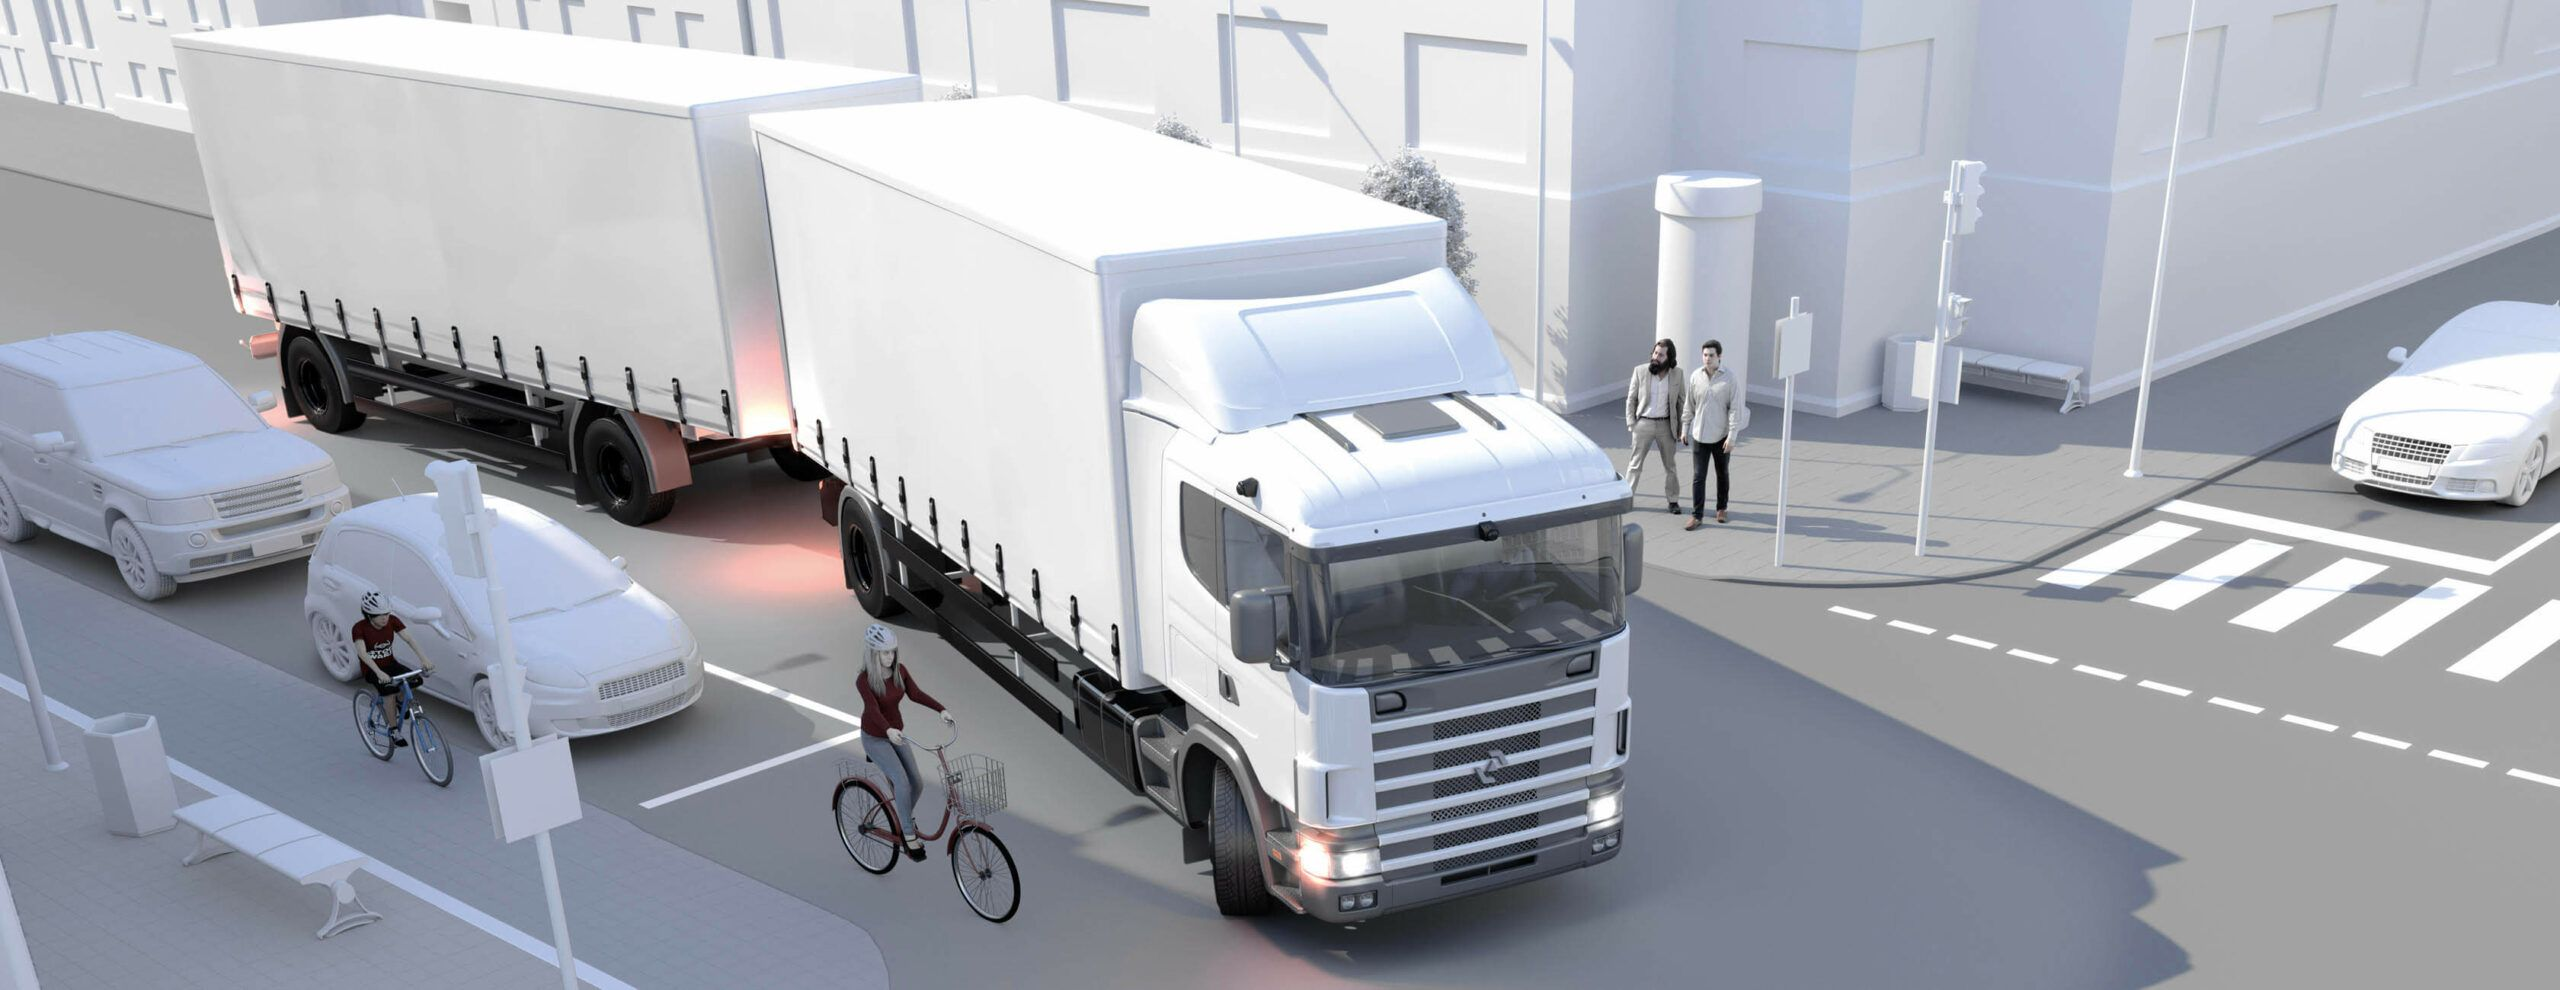
\includegraphics[width=\linewidth]{images/abbiegeassistent-scaled-7b2478b8}
  \caption{Rechtsabbiegesituation mit Abbiegeassistent \cite{abbiegeassistent-foerderung}}
  \label{fig:abbiegeassistent}
\end{figure}

Eine besonders wichtige Neuerung im Bereich der \acf{LKW}-Sicherheit sind Abbiegeassistenten. Sie reduzieren den toten Winkel und tragen so
 wesentlich dazu bei, Unfälle – insbesondere beim Rechtsabbiegen – zu vermeiden. Obwohl erste Systeme bereits im Einsatz sind, besteht weiterhin 
 erhebliches Potenzial für Verbesserungen. Vertiefte Forschung und Entwicklung im Bereich der Fahrerassistenz kann das allgemeine Verkehrsrisiko 
 weiter senken und die Verkehrssicherheit signifikant erhöhen \cite{SlightIncreaseNumber}.

\clearpage

\subsection{Zielsetzung}
Diese Studienarbeit verfolgt zwei Hauptziele: Erstens soll ein leistungsfähiger Datenlogger entwickelt werden, der Messwerte des 
Fahrerassistenzsystems systematisch und zuverlässig erfasst. Dadurch können mehrere Teammitglieder parallel mit authentischen Messdaten arbeiten,
 ohne dauerhaft auf die Hardware zugreifen zu müssen. Zweitens wird die bestehende Visualisierung überarbeitet, um Messergebnisse klarer und 
 übersichtlicher darzustellen. Die Kombination aus verbesserter Datenerfassung und optimierter Darstellung erleichtert zukünftige Analysen und Tests, 
 erhöht die Qualität der Positionsbestimmung und steigert die Effizienz des gesamten Entwicklungsprozesses – letztlich mit dem Ziel, 
 die Verkehrssicherheit weiter zu verbessern.

 \clearpage


\section{Rückblick auf das mobile Warnsystem}

\subsection{Konzept und Zielsetzung}
Die vorangegangene Studienarbeit hatte das Ziel, ein mobiles Warnsystem zu entwickeln, das Abbiegeunfälle zwischen \ac{LKW} und ungeschützten 
Verkehrsteilnehmenden – insbesondere Fußgänger*innen und Radfahrer*innen – minimiert.  
Kern des Ansatzes war eine Smartphone-Applikation, die als aktiver Bluetooth-Sender (Tag) fungiert. In Verbindung mit einem am \ac{LKW} montierten 
Empfängerboard (u-blox XPLR-AOA-1) sollte mithilfe der \acf{AoA}-Technologie die Position des Smartphones bestimmt und bei kritischen Situationen eine 
Warnung ausgegeben werden.  
Durch den Verzicht auf spezielle Hardware für die Verkehrsteilnehmenden versprach das System einen kostengünstigen und leicht zugänglichen Beitrag zur 
Verkehrssicherheit im urbanen Raum.

\subsection{Bluetooth-AoA – technische Grundlagen}
\ac{AoA} ist Bestandteil des Bluetooth-5.1-Standards. Mehrere Antennen auf dem Empfängerboard messen den Einfallswinkel des Funksignals; aus 
mindestens zwei Winkeln lässt sich per Triangulation die Position des Senders bestimmen \cite{miller2021bluetooth,uBloxAoAWhitepaper}.  
Voraussetzungen sind:

\begin{itemize}[leftmargin=2em]
  \item Zugriff auf die Sendeparameter des Bluetooth-Tags (z.\,B. Werbe­kanäle und Signalform),
  \item eine Antennenkonfiguration mit bekannten geometrischen Abständen,
  \item zeitlich hochaufgelöste Phasen- bzw. I/Q-Messungen im Empfänger.
\end{itemize}

Das u-blox XPLR-AOA-1 Explorer Kit erfüllt diese Bedingungen, da es sowohl ein \ac{AoA}-fähiges Empfängerboard als auch einen vorkonfigurierten 
Tag mitbringt. In der vorangegangenen Arbeit sollte das Smartphone diese Tag-Funktion übernehmen.

\begin{figure}[H]
  \centering
  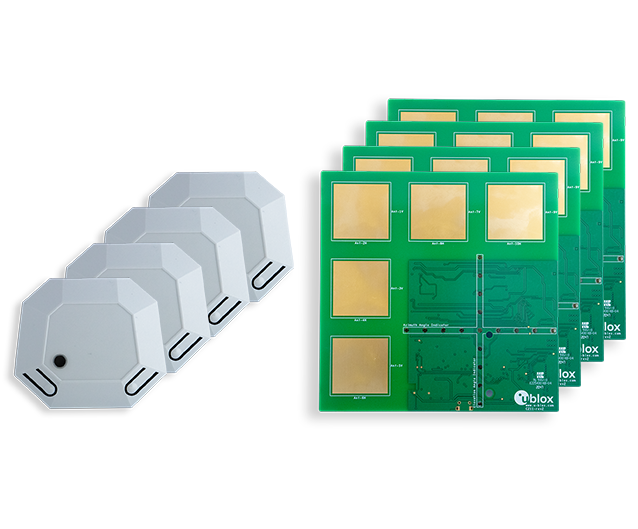
\includegraphics[width=\linewidth]{images/XPLR-AOA-with-C209-and-C211-02_0}
  \caption{u-blox XPLR-AOA-2 Explorer Kit \cite{u-blox-xplr-aoa2}}
  \label{fig:xplr-aoa}
\end{figure}

\subsection{Herausforderungen und Gründe für die Projektpause}
Im praktischen Versuch zeigten sich mehrere technische Hürden, die eine Fortführung des Projekts verhinderten:

\begin{itemize}[leftmargin=2em]
  \item \textbf{Eingeschränkter Bluetooth-Stack auf Smartphones:} Aktuelle Android-Firmware erlaubt keinen vollständigen Zugriff auf Low-Level-Sendeparameter. Ein gezieltes Aussenden der für \ac{AoA} nötigen \ac{BLE}-Werbepakete ist mit dem Standard-\ac{SDK} nicht möglich \cite{androidBLElimitation}.
  \item \textbf{Begrenzte Verfügbarkeit von Bluetooth 5.1:} Nur wenige Endgeräte unterstützen bislang den vollständigen 5.1-Funktionsumfang. Dies reduziert Reichweite und Genauigkeit der Ortung.
  \item \textbf{Fehlende Systemrechte:} Die Emulation des u-blox-Tags scheiterte an fehlendem Root-Zugriff sowie an nicht freigegebenen Low-Level-\ac{API}s.
\end{itemize}

Aufgrund dieser Limitierungen konnte das Projekt nicht wie geplant abgeschlossen werden. Die zugrunde liegende Idee bleibt jedoch 
vielversprechend und kann erneut aufgegriffen werden, sobald die Geräteunterstützung für Bluetooth 5.1 breiter verfügbar ist und Betriebssysteme 
einen tieferen Zugriff auf den Bluetooth-Stack erlauben.

\clearpage

\section{Grundlagen Datenlogger}

\subsection{Zweck und Funktionalität eines Datenloggers}
Ein Datenlogger ist ein autonom arbeitendes Gerät bzw. Software-Modul, das physikalische oder digitale Messwerte über einen definierten Zeitraum 
aufzeichnet.  
Ziel ist es, Veränderungen systematisch und zuverlässig zu erfassen, um sie später analysieren, auswerten oder dokumentieren zu 
können \cite{poole2020data,smith2018sensors}.  
Typische Messgrößen sind beispielsweise Temperatur, Spannung, Zeitstempel sowie Lage- oder Positionsdaten.

\begin{figure}[H]
  \centering
  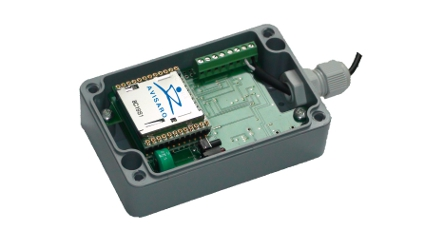
\includegraphics[width=\linewidth]{images/Datalogger}
  \caption{Datenlogger Cube (Avisaro 2.0) zur Speicherung von Sensor- und Prozessdaten \cite{wikipedia-datalogger}}
  \label{fig:datenlogger_cube}
\end{figure}

Im Unterschied zu interaktiven Messsystemen arbeitet ein Datenlogger in der Regel ohne permanente Verbindung zu einem Steuergerät.  
Damit eignet er sich besonders für mobile oder schwer zugängliche Anwendungen. Die kontinuierliche Aufzeichnung ermöglicht eine lückenlose 
Nachverfolgbarkeit und ist vor allem während Entwicklung, Fehlersuche und Validierung technischer Systeme von großer Bedeutung \cite{dewesoft2024guide}.

Wesentliche Eigenschaften eines Datenloggers sind eine ausreichende Speicherkapazität, hohe Energieeffizienz sowie die Kompatibilität zu 
standardisierten Datenformaten wie \ac{CSV} oder \ac{JSON}. Moderne Geräte bieten darüber hinaus Schnittstellen für drahtlose Datenübertragung 
oder eine automatisierte Synchronisation mit Analysetools \cite{rs2022guide}.

\subsection{Anwendungsbereiche im Kontext dieser Studienarbeit}
In dieser Arbeit wird der Datenlogger eingesetzt, um die Entwicklung des Bluetooth-\ac{AoA}-Lokalisierungssystems effizienter und flexibler zu gestalten.  
Während Test- und Optimierungsphasen soll die Abhängigkeit von einer Live-Verbindung zur Hardware minimiert werden \cite{poole2020data}.  
Entwickelnde können somit reale Messdaten analysieren, ohne direkt auf die u-blox-Hardware zugreifen zu müssen.

Der Logger speichert originalgetreue Messwerte, die anschließend in externe Werkzeuge importiert werden können, um Berechnungen, Analysen oder 
grafische Darstellungen vorzunehmen.  
Parameter- oder Algorithmus­änderungen lassen sich so anhand aufgezeichneter Daten überprüfen, ohne dass dafür eine erneute Datenerfassung 
erforderlich ist \cite{smith2018sensors}.

\begin{figure}[H]
    \centering
    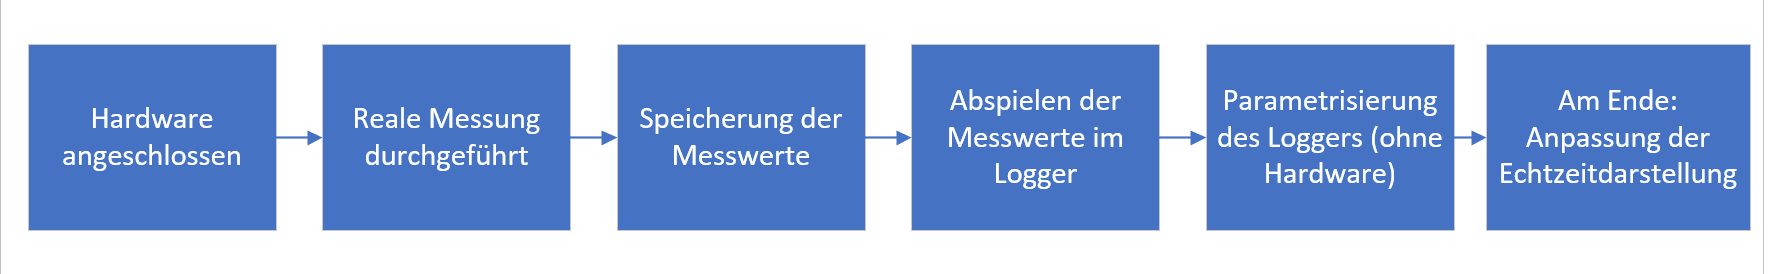
\includegraphics[width=\linewidth]{images/Flussdiagramm Datenlogger.png}
    \caption{Einbindung des Datenloggers in den Entwicklungsprozess\\
             Quelle: Eigene Darstellung}
    \label{fig:datenlogger_flow}
\end{figure}


Darüber hinaus ermöglicht der Datenlogger eine \emph{Offline-Simulation} beziehungsweise ein Daten-Replay mit realen Werten.  
Optimierungen können zunächst im Testsystem bewertet und erst bei zufriedenstellendem Ergebnis auf das reale System übertragen werden.  
Der Logger trägt somit wesentlich zur Entkopplung von Entwicklung und Hardwareverfügbarkeit bei.

\clearpage

\subsection{Herausforderungen und Lösungsansätze}
Bei der Entwicklung eines zuverlässigen Datenloggers für das Bluetooth-\ac{AoA}-System treten mehrere Herausforderungen auf:

\begin{itemize}[leftmargin=2em]
  \item \textbf{Zeitliche Synchronisation:} Für eine konsistente Auswertung müssen Zeitstempel, Empfangswinkel und weitere Messgrößen exakt zueinander passen \cite{rs2022guide}.
  \item \textbf{Speichereffizienz:} Große Datenmengen sollen verlustfrei, aber kompakt abgelegt werden. Ein strukturiertes Format wie \ac{CSV} oder \ac{JSON} erleichtert die spätere Analyse in Python oder MATLAB \cite{dewesoft2024guide}.
  \item \textbf{Integration in bestehende Prozesse:} Der Logger muss modular sein und sich ohne großen Aufwand in unterschiedliche Testumgebungen einfügen lassen. Ein niedriger Energieverbrauch ist dabei essenziell, um auch längere mobile Einsätze zu unterstützen \cite{smith2018sensors}.
\end{itemize}

Als Lösungsansätze dienen

\begin{itemize}[leftmargin=2em]
  \item die Verwendung eines einfachen, standardisierten Speicherformats,
  \item ein modular aufgebautes Software-Design mit klar dokumentierten Schnittstellen,
  \item sowie grundlegende Mechanismen zur Fehlererkennung und Datensynchronisation.
\end{itemize}

Diese Maßnahmen gewährleisten, dass der Datenlogger zuverlässig, energieeffizient und benutzerfreundlich eingesetzt werden kann \cite{poole2020data}.

\clearpage


%--------------------------------------------------------------------
\section{Entwicklung des Datenloggers}
%--------------------------------------------------------------------

\subsection{Anforderungen an die Software}
Die zu entwickelnde Datenlogger-Software muss sich nahtlos in die bestehende Systemarchitektur integrieren lassen und dabei drei Kernanforderungen 
erfüllen:

\begin{itemize}[leftmargin=2em]
  \item \textbf{Robuste Datenspeicherung} aller relevanten Messwerte,
  \item \textbf{flexible Wiederverwendung} der gespeicherten Daten für Tests und Visualisierungen,
  \item \textbf{einfache Wart- und Erweiterbarkeit} des Quellcodes.
\end{itemize}

Ein zentrales Ziel ist die \emph{Entkopplung} der Datenerfassung von der physischen Hardware.  
Durch die Offline-Nutzung gespeicherter Messreihen können Entwicklerinnen und Entwickler auch ohne Zugang zur u-blox-Hardware Analysen durchführen 
und Visualisierungen testen.  

Darüber hinaus wurde eine klar strukturierte, maschinenlesbare Datenhaltung gefordert, damit die aufgezeichneten Werte in gängigen Werkzeugen 
(z.\,B. Python, MATLAB) unmittelbar weiterverarbeitet werden können.  
Mehrbenutzerfähigkeit und Plattformunabhängigkeit gelten als wünschenswerte Eigenschaften.

%--------------------------------------------------------------------
\subsection{Auswahl geeigneter Technologien und Tools}
%--------------------------------------------------------------------
Die vorhandene Kommunikation mit der u-blox-Hardware basiert auf einer performanten \mbox{C++-Schicht}.  
Um diese beizubehalten und dennoch agile Erweiterungen zu ermöglichen, wurde eine zweistufige Architektur gewählt:

\begin{itemize}[leftmargin=2em]
  \item \textbf{C++}: bestehende, zeitkritische Kommunikation mit den Empfängerboards,  
  \item \textbf{Python}: neuer Datenlogger, Replay-Funktion und Visualisierung.
\end{itemize}

Diese Kombination vereint die Rechenleistung von C++ mit der Entwicklungsproduktivität von Python \cite{cpp_python_integration}.

Als Speicherformat kommt \ac{JSON} zum Einsatz, genauer das \acf{JSONL}-Format.  
Es gestattet, komplexe Datensätze – Zeitstempel, \ac{AoA}-Winkel, Signalstärken und Metadaten – zeilenweise abzulegen, maschinenlesbar zu 
versionieren und später sequentiell einzulesen \cite{json_logging_bestpractices}.  

Die in Abschnitt 4.1 genannten Anforderungen werden damit erfüllt: Die Lösung ist plattformunabhängig, modular 
und teamfreundlich.

%--------------------------------------------------------------------
\subsection{Implementierung und Integration in das bestehende System}
%--------------------------------------------------------------------
Das Lokalisierungssystem basiert auf der Bluetooth-\ac{AoA}-Technologie.  
Der Datenfluss wurde so gestaltet, dass Messung, Speicherung und Analyse wahlweise live oder offline erfolgen können.

\paragraph{Messung – Entstehung der Rohdaten}
\begin{itemize}[leftmargin=2em]
  \item \textbf{Tag}: sendet kontinuierlich Bluetooth-Signale.  
  \item \textbf{Anker} (mind.\ zwei): empfangen die Signale mit Mehrantennen-Arrays und bestimmen die Einfallswinkel~(\ac{AoA}).
\end{itemize}

\paragraph{Datenerfassung und -aufbereitung}
Ein Python-Skript (\texttt{getAnchorData.py} \cite{tadic-studienarbeit-ui}) liest die Rohdaten über eine serielle Schnittstelle bzw. \ac{BLE} aus.  
Pro Messzyklus werden unter anderem

\begin{itemize}[leftmargin=2em]
  \item \texttt{anchors} (Koordinaten der Anker), 
  \item \texttt{angles} (gemessene Winkel) sowie
  \item \texttt{sensor\_values} (weitere Metadaten)
\end{itemize}

in eine \texttt{.jsonl}-Datei geschrieben. Jede Zeile enthält einen ISO-Zeitstempel und das zugehörige Messobjekt.

\paragraph{Berechnung der Tag-Position – Triangulation}
Aus zwei Winkelmessungen und den bekannten Ankerpositionen lässt sich die Tag-Position über Triangulation bestimmen.  
Für jeden Anker $i$ gilt mit Winkel~$\theta_i$ der Richtungsvektor
\[
  \vec d_i = \bigl(\sin\theta_i,\; \cos\theta_i\bigr).
\]
Schneidet man die durch $(x_i,y_i)$ mit Richtung $\vec d_i$ definierten Geraden, erhält man
\[
  t_1 = \frac{(x_2-x_1) \, d_{y,2} - (y_2-y_1) \, d_{x,2}}{d_{x,1} \, d_{y,2} - d_{y,1} \, d_{x,2}},\qquad
  \vec p = (x_1,y_1) + t_1 \, \vec d_1 .
\]
Die Berechnung erfolgt wahlweise \emph{live} oder später im Replay-Modus.

\begin{figure}[H]
  \centering
  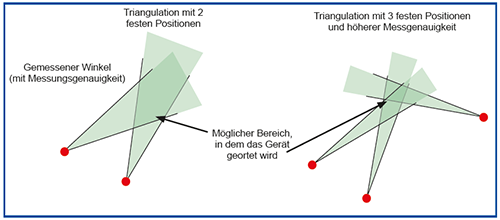
\includegraphics[width=\linewidth]{images/1906_abbildung1.png}
  \caption{Beispielhafte Triangulation \cite{comconsult-wlan-ortung}}
  \label{fig:triangulation_example}
\end{figure}


\paragraph{Speicherung und Wiederverwendung}
Alle berechneten Werte werden chronologisch gespeichert.  
Das Skript \texttt{replayLogger.py \cite{tadic-studienarbeit-ui}} liest die Logdatei ein, berechnet bei Bedarf die Position neu und stellt die Daten über 
eine \acf{TCP}-Schnittstelle der Visualisierung (\texttt{ui.py} \cite{tadic-studienarbeit-ui}) bereit.

\begin{figure}[H]
    \centering
    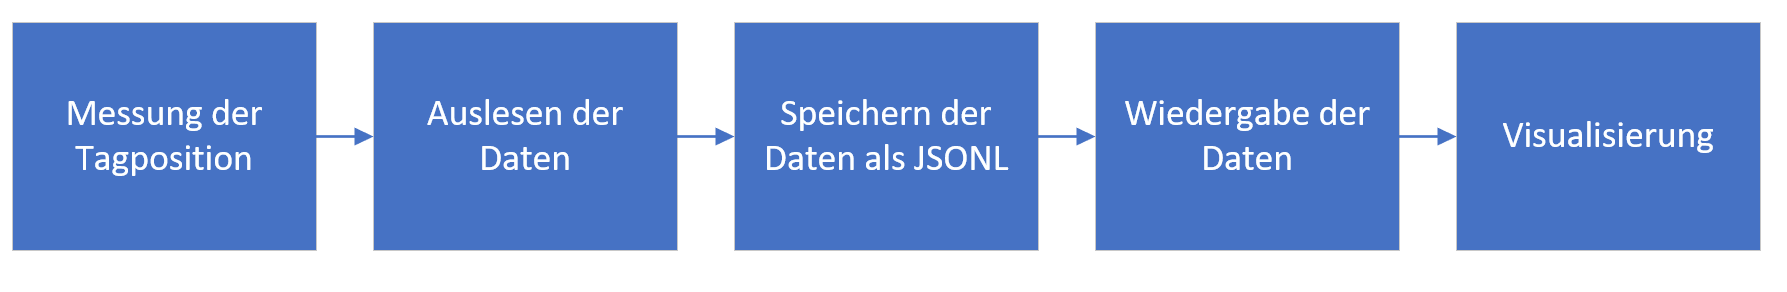
\includegraphics[width=\linewidth]{images/Ablauf Funktion Datenlogger.png}
    \caption{Gesamter Datenfluss vom Messvorgang bis zur Visualisierung\\
            Quelle: Eigene Darstellung}
    \label{fig:datenlogger_flow_impl}
\end{figure}

\paragraph{Nachträgliche Optimierung}
Frühe Versionen spielten im Replay nur die gespeicherten Koordinaten ab.  
Das Modul wurde daher erweitert, sodass beim Einlesen stets aus den Rohwinkeln \textit{neu} trianguliert wird.  
Somit lassen sich Algorithmen offline verifizieren, bevor sie in das Echtzeitsystem übernommen werden.

\paragraph{Visualisierung}
Die \ac{TCP}-Schnittstelle sendet jede Messung als \ac{JSON}-Objekt an die \acf{UI}.  
Dort werden Tag-Position, Anker, Bewegungsrichtung und Risikostufe live angezeigt.

\clearpage

\paragraph{Zusammenfassung des Datenflusses}
\begin{enumerate}[leftmargin=2em]
  \item \textbf{Messung} – Anker erfassen Winkel und Sensordaten.  
  \item \textbf{Logging} – Python-Skript speichert Messwerte Zeile für Zeile in \texttt{.jsonl}.  
  \item \textbf{Replay} – \texttt{replayLogger.py \cite{tadic-studienarbeit-ui}} liest Daten, trianguliert erneut und streamt sie.  
  \item \textbf{Visualisierung} – \texttt{ui.py \cite{tadic-studienarbeit-ui}} stellt Position und Zusatzinfos dar.
\end{enumerate}

%--------------------------------------------------------------------
\subsection{Ergebnisse und Evaluation}
%--------------------------------------------------------------------
Der Datenlogger ließ sich mit wenigen Code-Ergänzungen in die bestehende Software integrieren.  
Die Lösung

\begin{itemize}[leftmargin=2em]
  \item erfasst Messdaten zuverlässig,
  \item speichert sie zeilenweise im \texttt{.jsonl}-Format,
  \item ermöglicht ein hardwareunabhängiges Replay,
  \item und überträgt die Daten stabil per \ac{TCP} an die \ac{UI}.
\end{itemize}

Zur komfortablen Bedienung wurde eine \texttt{.bat}-Datei bereitgestellt, die den Logger startet und aufgezeichnete Datensätze zur Auswahl stellt.  
Mehrere Teammitglieder können so parallel mit denselben Messdaten arbeiten – unabhängig von der Hardwareverfügbarkeit.

Erste Tests mit kurzen bis mittellangen Aufzeichnungen (mehrere Minuten) verliefen problemlos.  
Für den Produktiveinsatz sind Langzeittests vorgesehen, um Speicherstabilität und Performance bei großen Datenmengen zu validieren.

\begin{figure}[H]
    \centering
    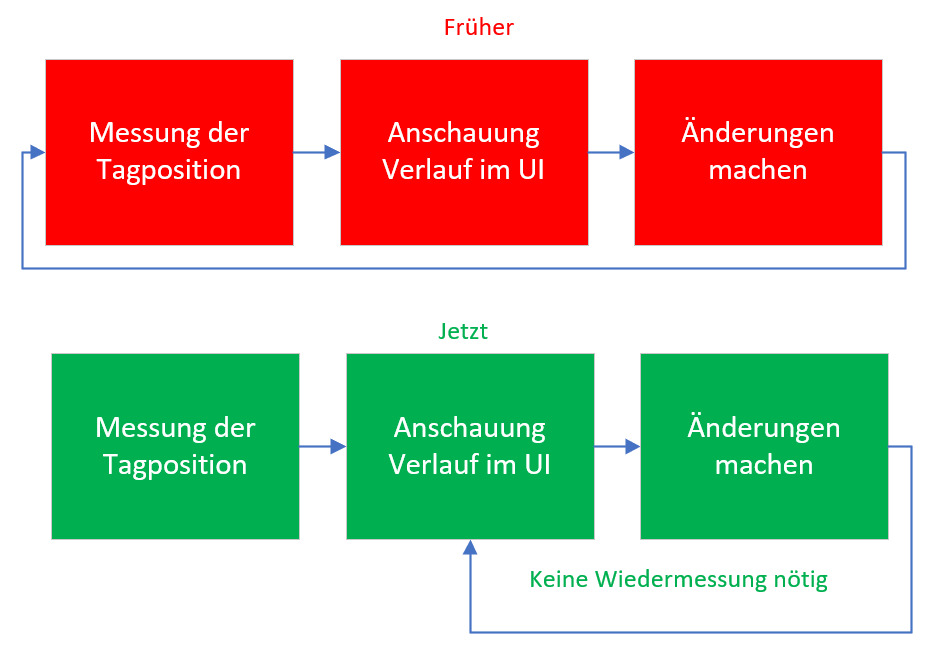
\includegraphics[width=\linewidth]{images/Vergleich Parametrisierung.png}
    \caption{Parametrierung ohne (links) und mit (rechts) Datenlogger-Workflow\\
            Quelle: Eigene Darstellung}
    \label{fig:parameter_comparison}
\end{figure}

\noindent
Der entwickelte Logger bildet somit eine stabile Grundlage für künftige Entwicklungs- und Testarbeiten und trägt wesentlich zu effizienteren, 
hardware­unabhängigen Validierungsprozessen bei.

\clearpage


%--------------------------------------------------------------------
\section{Grundlagen der Visualisierung}
%--------------------------------------------------------------------

\subsection{Anforderungen an eine effektive Visualisierung}

Die visuelle Aufbereitung von Mess- und Sensordaten ist ein zentrales Element der Systementwicklung.  
In dieser Studienarbeit dient die Visualisierung nicht allein als Ausgabe­instrument, sondern als aktives \emph{Analysewerkzeug}. Daraus ergeben sich spezifische Anforderungen an Struktur, Funktionalität und Performance:

\begin{description}[style=nextline,leftmargin=2em]
  \item[Klarheit und Verständlichkeit]  
        Tag-Position, Winkelmessungen sowie Zusatz­informationen (z.\,B. Risikostufe) müssen intuitiv erfassbar sein und dürfen keine unnötige Komplexität erzeugen.
  \item[Reaktionsfähigkeit]  
        Insbesondere beim Replay ist eine quasi­echtzeit­fähige Darstellung erforderlich, damit zeitkritische Situationen nachvollziehbar bleiben.
  \item[Strukturierte, modulare Ebenen]  
        Anker­positionen, Trajektorien, Messwinkel und Risikoindikatoren werden auf separaten Layern visualisiert; eine Farb- oder Symbol­codierung erleichtert das Erkennen von Korrelationen.
  \item[Konfigurierbarkeit]  
        Parameter und Daten­sätze müssen sich flexibel umschalten lassen, um unterschiedliche Szenarien vergleichen und analysieren zu können.
  \item[Stabilität \& Performance]  
        Auch bei großen Datenmengen darf die Oberfläche weder verzögert reagieren noch hohe Systemressourcen beanspruchen.
  \item[Schnittstellen­kompatibilität]  
        Die \ac{UI} empfängt Daten kontinuierlich per \ac{TCP} in \ac{JSON}-Struktur; eingehende Pakete sind verlustfrei zu dekodieren und anzuzeigen.
  \item[Benutzerfreundliche Interaktion]  
        Eine klare Bedienlogik ermöglicht auch neuen Teammitgliedern oder externen Testern einen schnellen Einstieg.
\end{description}

%--------------------------------------------------------------------
\subsection{Darstellungsformen und Technologien}
%--------------------------------------------------------------------

\paragraph{2D-Darstellung}

Ein kartesisches Koordinatensystem bildet die Basis:  
Anker werden als feste Punkte eingezeichnet, die aktuelle Tag-Position als Marker (ggf. farblich kodiert: Grün\,=\,sicher, Gelb\,=\,Warnung, Rot\,=\,Kollisionsgefahr).
Sensorlinien oder Vektorpfeile verdeutlichen gemessene Winkel und Gefahrenzonen.  
Ein Replay-Modus zeigt frühere Positionen sequenziell an und gestattet so die Analyse von Bewegungs­mustern.

\paragraph{Technische Umsetzung}

\begin{itemize}[leftmargin=2em]
  \item \textbf{Python / Tkinter} – leichtgewichtige \ac{UI}, Canvas-Zeichenfläche für dynamische Objekte \cite{tkinter_book}. 
  \item \textbf{\ac{TCP}} – kontinuierlicher Datenstrom vom Logger zur \ac{UI} (Modul \texttt{ui.py}).
  \item \textbf{\ac{JSON}-Parsing} – Dekodierung der Log- und Live-Pakete.
\end{itemize}

Die modulare Struktur erlaubt spätere Migration zu \texttt{PyQt}, \texttt{Plotly Dash} oder 3D-Frameworks (OpenGL, Unity), ohne die Backend-Logik anzutasten.

\paragraph{Schnittstellen \& Erweiterbarkeit}

Neben Live-Daten unterstützt die Oberfläche einen reinen Replay-Betrieb. Ein Startskript (Batch oder CLI-Parameter) wählt die gewünschte Logdatei.  
Backend (Logger\,/\,Replay) und Frontend (\ac{UI}) sind klar getrennt; neue Sensorquellen lassen sich per standardisiertem \ac{JSON}-Schema einbinden.

\paragraph{Empfohlene Übersichtsgrafik (optional)}

Eine schematische Abbildung kann den vollständigen Visualisierungs­pfad veranschaulichen:

\begin{itemize}[leftmargin=2em]
  \item Anker-Positionen als fixe Punkte  
  \item Messwinkel als Richtungslinien  
  \item Tag-Marker mit Zeitstempel  
  \item Farbring für Risikostufe  
  \item Bewegungspfad (gestrichelte Linie)
\end{itemize}

Solch eine Grafik erleichtert auch fachfremden Stakeholdern das Verständnis des Systems.

\paragraph{Fazit}

Die gewählten Technologien liefern eine performante, verständliche und erweiterbare Visualisierung.  
Sie bilden damit eine solide Grundlage für die weiterführende Analyse, Parametrierung und Validierung des Fahrerassistenzsystems.

\clearpage


\section{Entwicklung der neuen Visualisierung}
\subsection{Analyse der bestehenden Visualisierung}

Die bisherige grafische Benutzeroberfläche (\ac{UI}) wurde in Python entwickelt und diente der Echtzeitdarstellung der aus dem Bluetooth-\ac{AoA}-System ermittelten
Tag-Position. Als zentrales Element wurde ein zweidimensionales kartesisches Koordinatensystem verwendet, innerhalb dessen ein einzelner Punkt die 
Bewegung des Tags repräsentierte. Die Position dieses Punktes wurde entweder durch eine direkte Live-Messung mit der Hardware oder durch eine 
vereinfachte Simulation erzeugt – eine Möglichkeit zur Wiederverwendung gespeicherter Daten durch einen Datenlogger war zu diesem Zeitpunkt noch nicht
implementiert \cite{tkinter_book}.

\begin{figure}[H]
    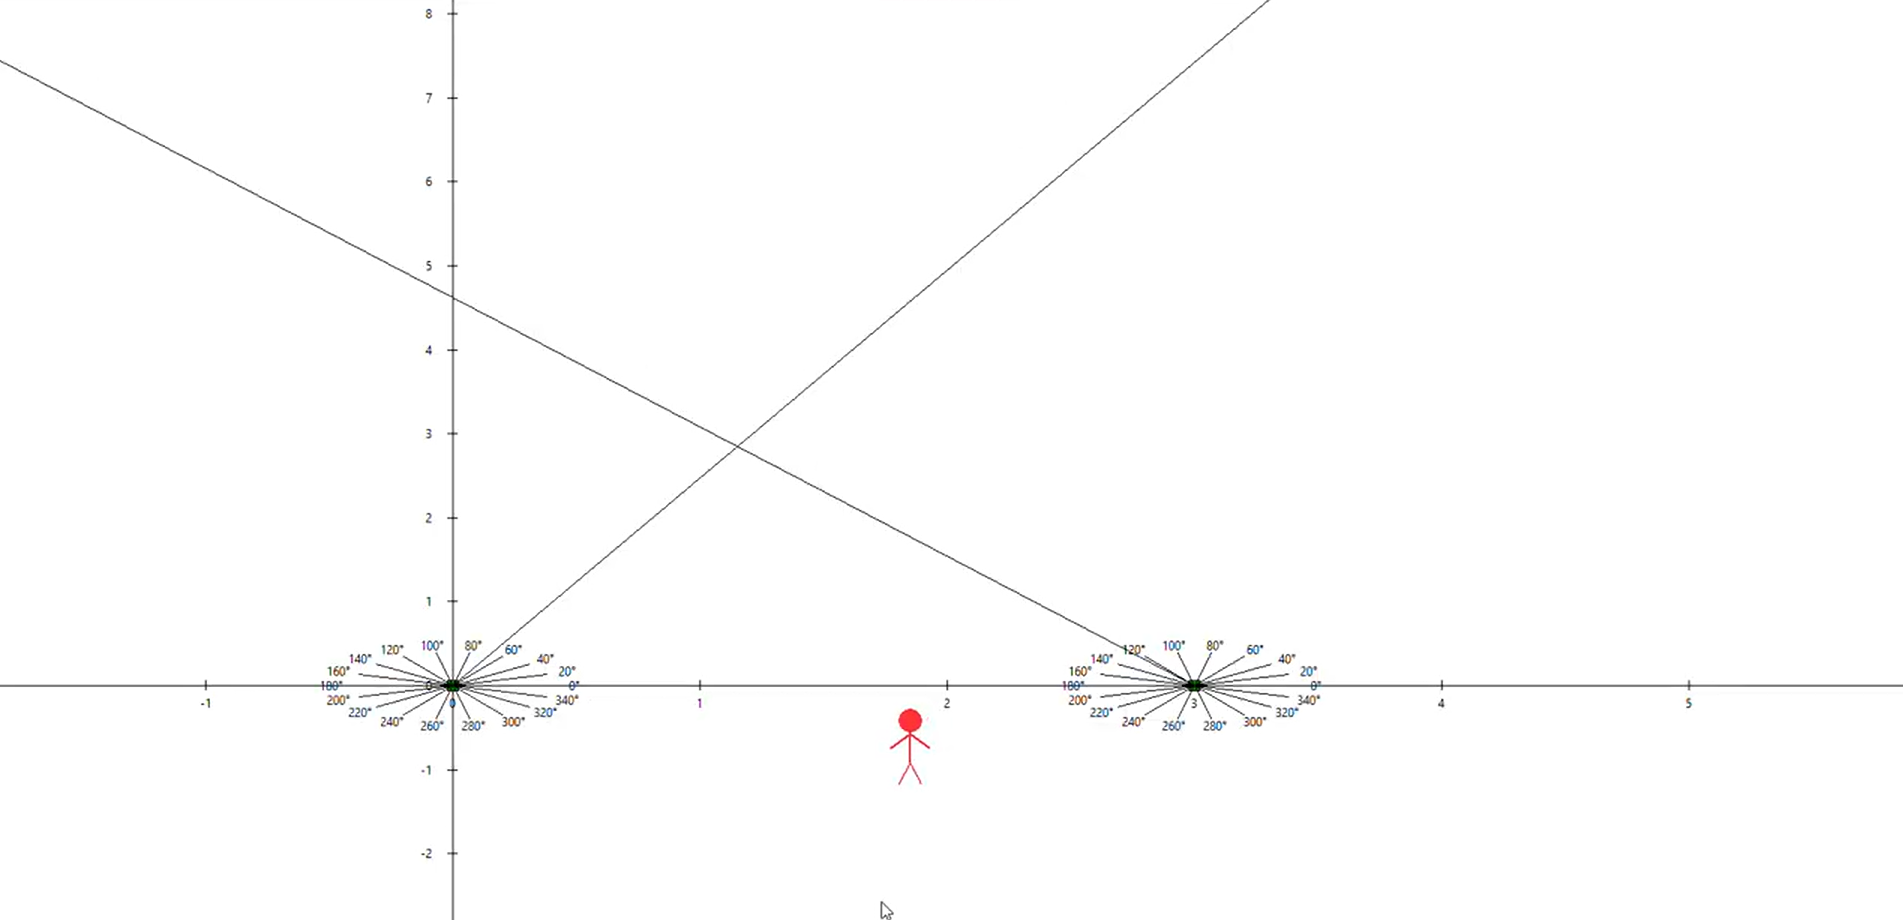
\includegraphics[width=1\linewidth]{images/Alte Visualisierung.png}\\[1ex]
    \centering
    \caption{Alte Visualisierung \cite{tadic-studienarbeit-ui}}
    \label{ABBILDUNG}
\end{figure}

Zur besseren Nachvollziehbarkeit der geometrischen Zusammenhänge wurden auch die fest installierten Empfangseinheiten (Anker) im Koordinatensystem 
visualisiert. Von deren Positionen ausgehend wurden Linien gezeichnet, welche die gemessenen Einfallswinkel (\ac{AoA}) darstellten. Die 
Idee dahinter war, die Triangulation – also die Schnittpunktberechnung zweier Richtungslinien – visuell darzustellen und die damit berechnete Tag-Position
zu validieren.

Allerdings wies diese Darstellung mehrere funktionale und darstellerische Einschränkungen auf. Eine grundlegende Schwäche bestand darin, dass der 
dargestellte Schnittpunkt der Winkel-Linien oft nicht exakt mit dem angezeigten Punkt des Tags übereinstimmte. Dies führte zu Inkonsistenzen, die 
insbesondere bei der Bewertung der Lokalisierungsgenauigkeit zu Verwirrung führen konnten.

Darüber hinaus fehlten wichtige Interaktionsmöglichkeiten und Darstellungsmodi: Sensorwerte oder Risikobewertungen konnten 
nicht separat angezeigt oder analysiert werden. Eine Zeitschrittsteuerung oder ein Replay-Modus waren nicht vorhanden. Da der 
Datenlogger zum damaligen Zeitpunkt noch nicht existierte, beschränkte sich die Funktionalität der Oberfläche auf Live-Datenströme oder manuell 
eingespeiste Simulationsdaten.

Zusammenfassend war die ursprüngliche Visualisierung funktional auf das Wesentliche reduziert, ermöglichte aber weder eine tiefere Analyse noch eine 
Nachbearbeitung historischer Messdaten. Die Einführung des Datenloggers und eine verbesserte Visualisierung sollen diese Defizite beheben und eine 
fundierte, nachvollziehbare sowie interaktive Darstellung aller relevanten Systemparameter ermöglichen.

\subsection{Konzept einer verbesserten Visualisierung}

Basierend auf der Analyse der bisherigen Darstellung ergeben sich mehrere Ansatzpunkte für eine funktional und ästhetisch verbesserte Visualisierung
der Tag-Ortung. Ziel ist es, die Ausgabe so zu gestalten, dass auch technisch weniger versierte Personen – beispielsweise Besucher auf Messen oder 
Mitglieder in interdisziplinären Projektteams – intuitiv die Funktionsweise und Aussagekraft des Fahrerassistenzsystems nachvollziehen können.

Ein zentrales Element der neuen Visualisierung ist die verbesserte Darstellung des Tags. Bisher wurde dieser lediglich als bewegender Punkt im 
Koordinatensystem dargestellt, was der realen Anwendung – z.\,B. einem Fußgänger oder Fahrradfahrer im Straßenverkehr – kaum gerecht wurde. Zukünftig 
soll der Tag durch ein erkennbares Modell wie etwa eine stilisierte menschliche Figur (z.\,B. ein Stickman) ersetzt werden. Zusätzlich ist vorgesehen,
visuelle Elemente wie ein \ac{LKW}-Modell in die Darstellung zu integrieren, um die reale Gefahrenlage bei Abbiegesituationen plausibler zu simulieren.

Zur Verbesserung der Verständlichkeit soll die Bewegung des Tags flüssiger und zeitlich realistischer erfolgen. In der bisherigen Version war die 
Bewegung teils sprunghaft oder verzögert, was eine genaue Nachverfolgung erschwerte. Durch optimierte Synchronisation mit 
den übermittelten Messwerten soll die visuelle Bewegung stärker der tatsächlichen Bewegung des realen Objekts entsprechen.

Darüber hinaus ist geplant, ein interaktives Interface mit zusätzlichen Informationen bereitzustellen. So sollen Parameter wie Winkel, 
Positionskoordinaten oder Risikoindikatoren dynamisch eingeblendet und aktualisiert werden können – ein wesentliches Werkzeug für Entwickler bei der Fehleranalyse und Parametrierung.

Ein weiterer Aspekt der verbesserten Darstellung betrifft das bisher fest eingeblendete Koordinatensystem. Dieses war zwar funktional nützlich,
beeinträchtigte jedoch stellenweise die Lesbarkeit und ästhetische Wirkung der grafischen Oberfläche – insbesondere bei öffentlichkeitswirksamen 
Präsentationen oder auf begrenzten Anzeigeflächen. Künftig soll daher eine Option implementiert werden, das Koordinatensystem bei Bedarf auszublenden 
oder gezielt ein- und auszublenden (Toggle-Funktion). Dies erlaubt eine flexiblere Darstellung und steigert die Übersichtlichkeit – insbesondere wenn 
die rein visuelle Wahrnehmung im Vordergrund stehen soll.

Insgesamt verfolgt das neue Visualisierungskonzept das Ziel, eine Brücke zwischen technischer Präzision und intuitiver Darstellbarkeit zu schlagen. 
Es soll nicht nur die Qualität der Entwicklung verbessern, sondern auch die Kommunikation der Systemfunktionalität nach außen erleichtern – etwa in 
Präsentationen, bei Tests oder in zukünftigen Messen.

\subsection{Implementierung der verbesserten Visualisierung}

Zur besseren Nachvollziehbarkeit der gemessenen Bewegungsdaten und zur verständlichen Darstellung des Systems für technische wie nicht-technische 
Betrachter wurde die Benutzeroberfläche (\ac{UI}) umfassend überarbeitet. Die Implementierung erfolgte in Python unter Verwendung des 
\texttt{tkinter}-Frameworks, wodurch eine flexible und plattformunabhängige grafische Visualisierung ermöglicht wurde \cite{tkinter_book}.

\paragraph{Grundstruktur und Aufbau}

Die Benutzeroberfläche besteht aus einem zentralen Zeichenbereich (Canvas), auf dem die Bewegung des zu lokalisierenden Objekts (Tag) visualisiert wird. 
Ergänzt wird dieser durch eine Steuerleiste am unteren Rand zur Interaktion (z.\,B. Start/Stop der Visualisierung oder Ein-/Ausblenden von Antennendaten) 
sowie einer Informationsleiste zur Anzeige der aktuellen Position und Zusatzdaten.

Die Visualisierung ist in mehreren Schichten aufgebaut:
\begin{itemize}
    \item Darstellung des Tags als dynamisch skalierbare Figur (z.\,B. Stickman oder Fahrzeugabbildung)
    \item Hintergrundkoordinatensystem mit optional einblendbaren Achsen und Skalen
    \item Einblendung der Position und Orientierung der Antennenarrays sowie der zugehörigen Messrichtungen (\ac{AoA}-Linien)
\end{itemize}

\paragraph{Verarbeitung eingehender Daten}

Die Visualisierung kommuniziert über eine \ac{TCP}-Verbindung mit dem Datenlogger, der kontinuierlich strukturierte \ac{JSON}-Datenpakete sendet. Diese enthalten 
Informationen zur geschätzten Position des Tags, Sensordaten sowie Metainformationen. Eine dedizierte Serverkomponente in der \ac{UI} nimmt die Daten entgegen,
extrahiert relevante Parameter und aktualisiert die grafische Darstellung entsprechend.

Zur Verbesserung der Darstellung wurde ein Glättungsverfahren mit exponentiellem Filter implementiert, um Positionssprünge durch Rauschen oder Ausreißer 
zu reduzieren. Gleichzeitig werden unrealistische Sprünge oder abrupte Änderungen durch Grenzwerte abgefangen.

\paragraph{Darstellungskonzept des Tags}

Anstelle eines einfachen Punkts wird das Tag nun als abstrahierte Figur (Stickman) dargestellt. Diese passt sich dynamisch in Größe und Farbe an
den Abstand zu den Antennen an, um Nähe, Risiko oder Interaktionszonen visuell hervorzuheben. Alternativ kann ein repräsentatives Fahrzeugmodell 
(ein \ac{LKW}-Bild) eingebunden werden, um reale Szenarien wie Fahrassistenzsysteme intuitiver zu vermitteln.

\begin{figure}[H]
    \includegraphics[width=0.8\linewidth]{images/Stickman Grün.png}\\[1ex]
    \centering
    \caption{Grün - keine Gefahr noch \cite{tadic-studienarbeit-ui}}
    \label{ABBILDUNG}
\end{figure}
\begin{figure}[H]
    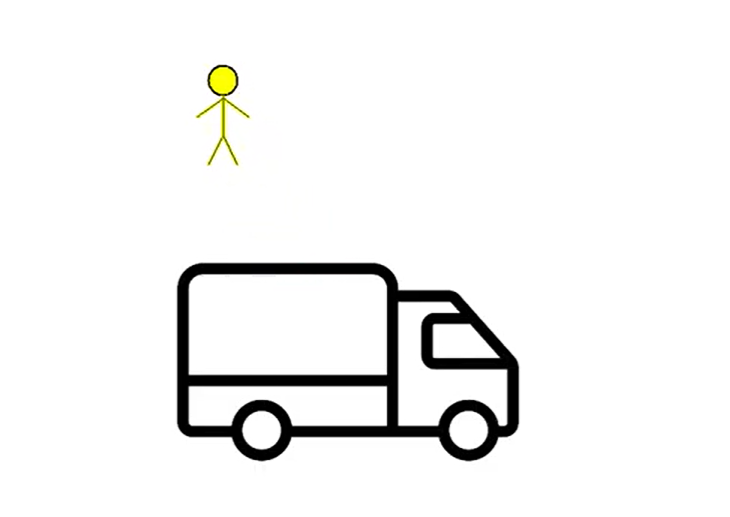
\includegraphics[width=0.8\linewidth]{images/Stickman Gelb.png}\\[1ex]
    \centering
    \caption{Gelb - Warnung, Gefahr möglich \cite{tadic-studienarbeit-ui}}
    \label{ABBILDUNG}
\end{figure}
\begin{figure}[H]
    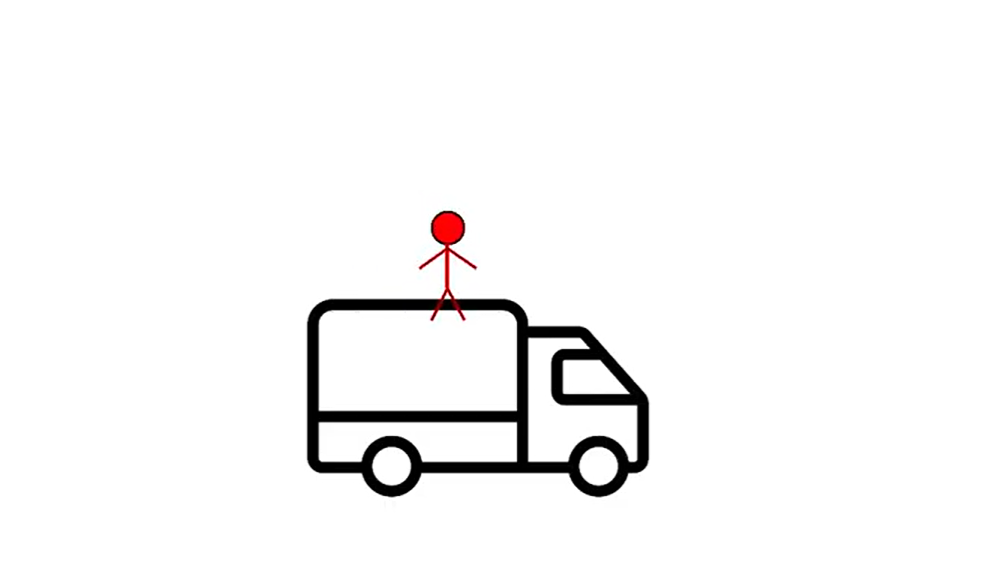
\includegraphics[width=1\linewidth]{images/Stickman Rot.png}\\[1ex]
    \centering
    \caption{Rot - Achtung, Kollisionsgefahr \cite{tadic-studienarbeit-ui}}
    \label{ABBILDUNG}
\end{figure}

\paragraph{Visualisierung der Antennen und Sensorlinien}

Die Position der Antennenarrays wird grafisch dargestellt und durch Linien ergänzt, welche die gemessenen Einfallswinkel (\ac{AoA}) andeuten. Diese Linien 
zeigen die theoretische Messrichtung, was ein besseres Verständnis der Triangulation erlaubt.

\begin{figure}[H]
    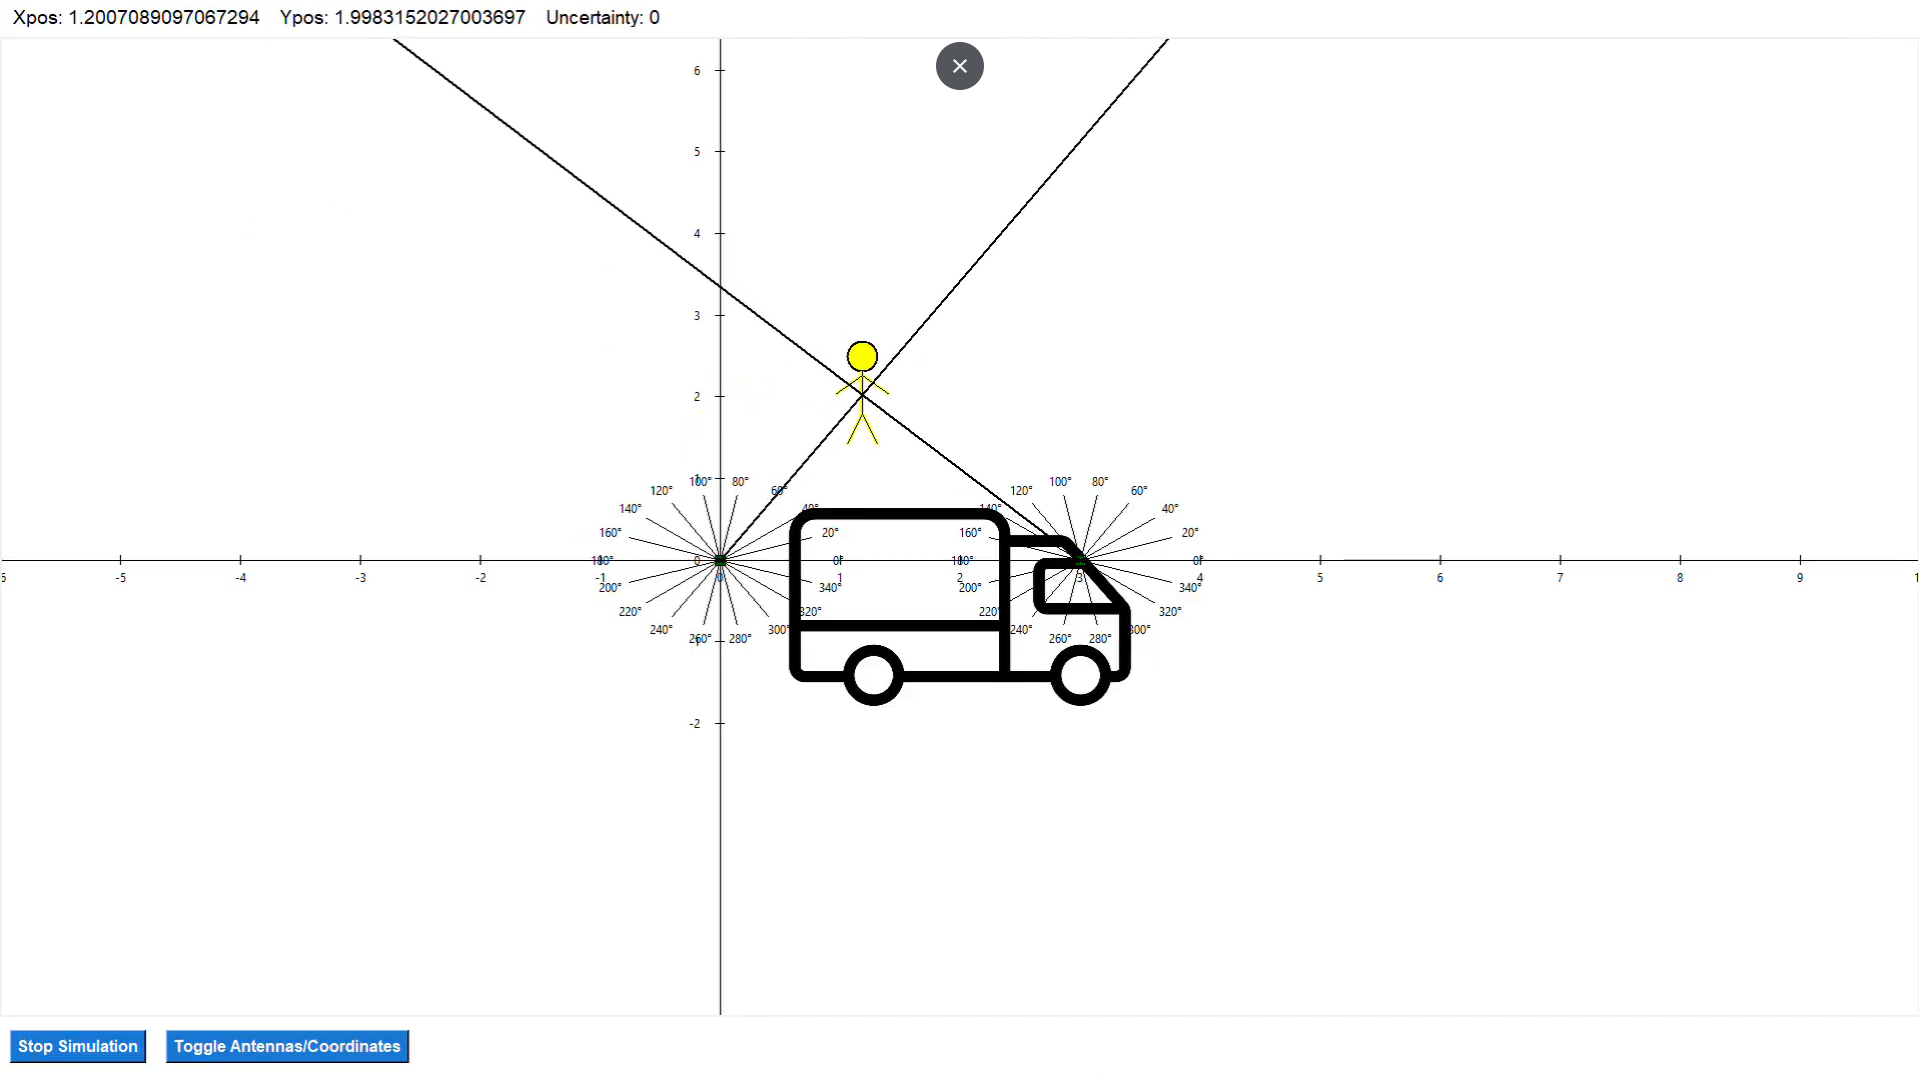
\includegraphics[width=1\linewidth]{images/Visualisierung Antennen.png}\\[1ex]
    \centering
    \caption{Visualisierung der Antennen und Sensorlinien \cite{tadic-studienarbeit-ui}}
    \label{ABBILDUNG}
\end{figure}

\paragraph{Interaktive Steuerung und Optimierungen}

Ein zentrales Element ist die Möglichkeit, zwischen verschiedenen Visualisierungsmodi umzuschalten. Über ein Toggle-Button kann die Darstellung der 
Koordinatenachsen und Sensorlinien aktiviert oder ausgeblendet werden, um je nach Anwendungsfall zwischen technischer Analyse und Präsentation zu 
wechseln. Zusätzlich kann die Darstellung bei Bedarf in den Vollbildmodus gesetzt werden.

Zur Steuerung und flexiblen Nutzung wurde außerdem eine ausführbare Batch-Datei (\texttt{.bat}) bereitgestellt, mit der definierte Logdateien gezielt 
abgespielt und getestet werden können. Diese Struktur erlaubt es, mehrere gespeicherte Datensätze individuell zu benennen, abzurufen und ohne 
Hardwarebezug zu analysieren.

\begin{figure}[H]
    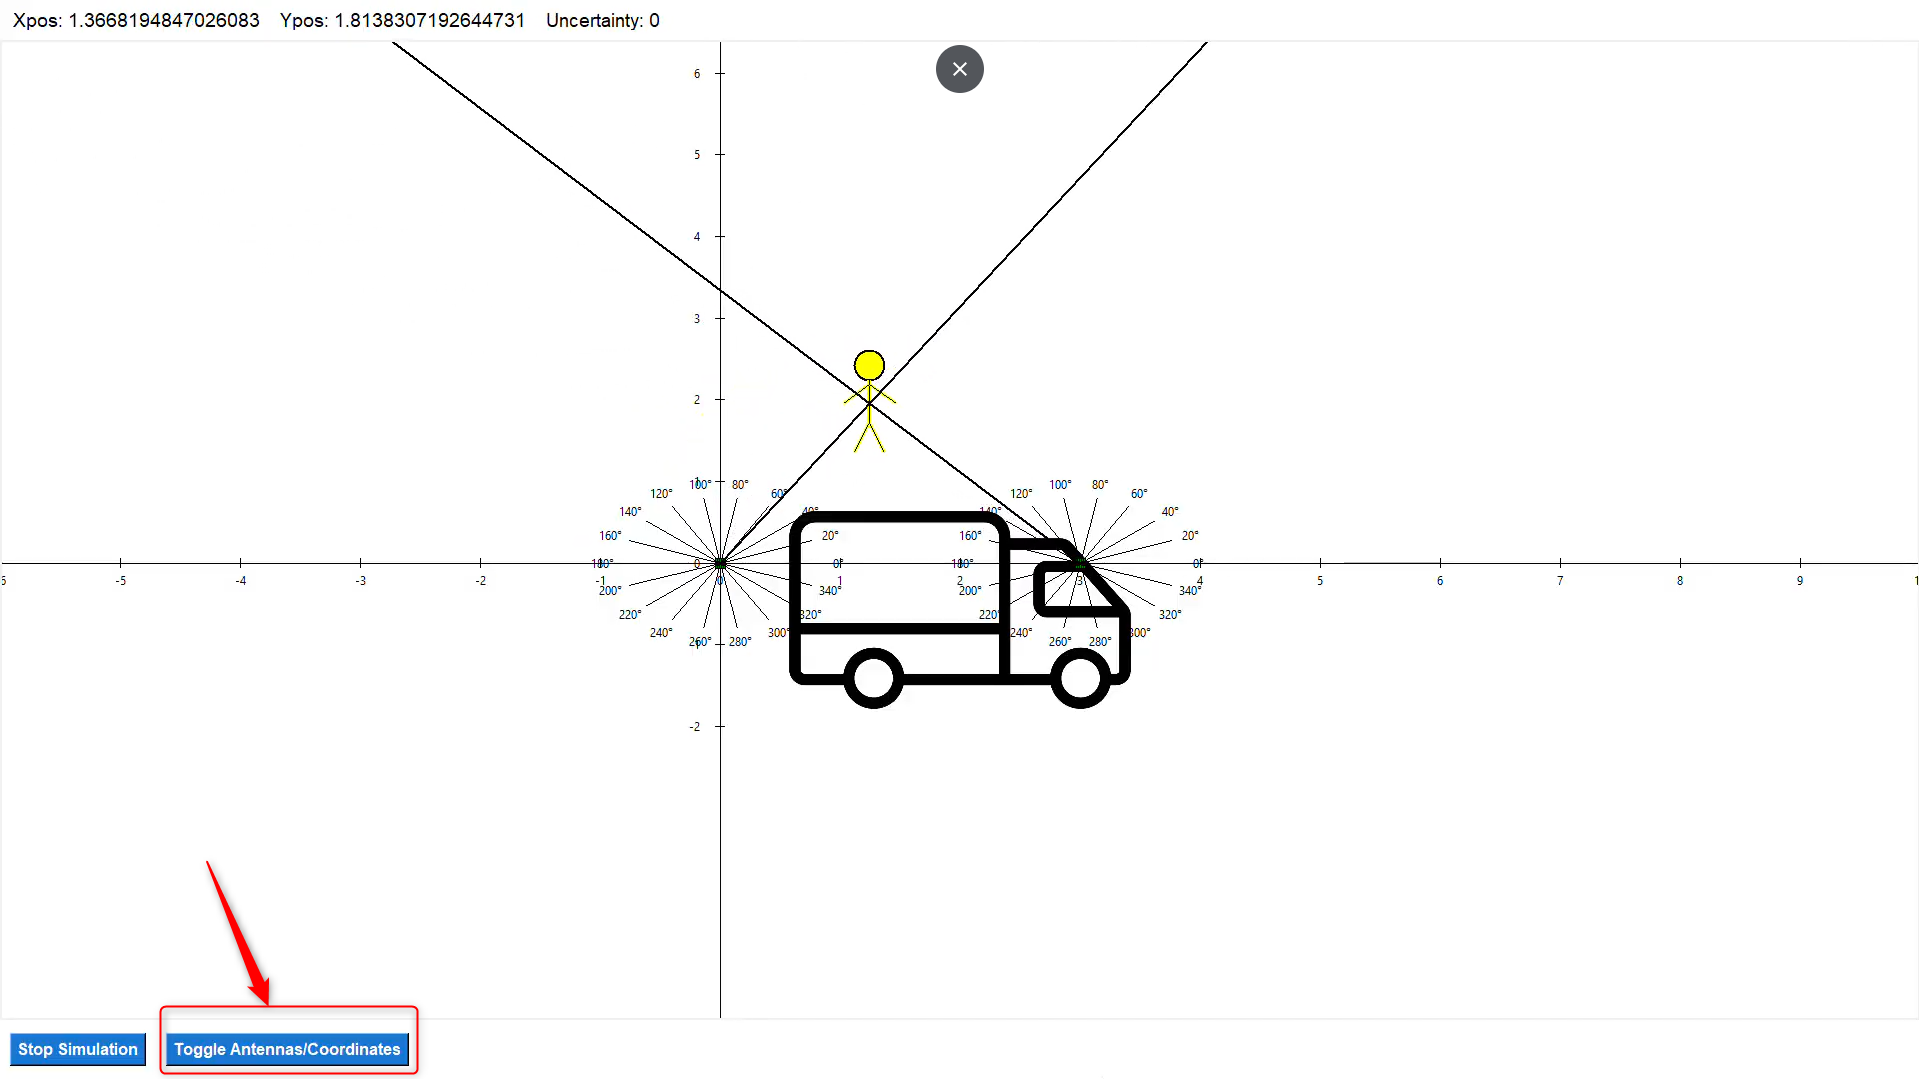
\includegraphics[width=1\linewidth]{images/Volle Darstellung.png}\\[1ex]
    \centering
    \caption{Volle Darstellung Benutzeroberfläche \cite{tadic-studienarbeit-ui}}
    \label{ABBILDUNG}
\end{figure}
\begin{figure}[H]
    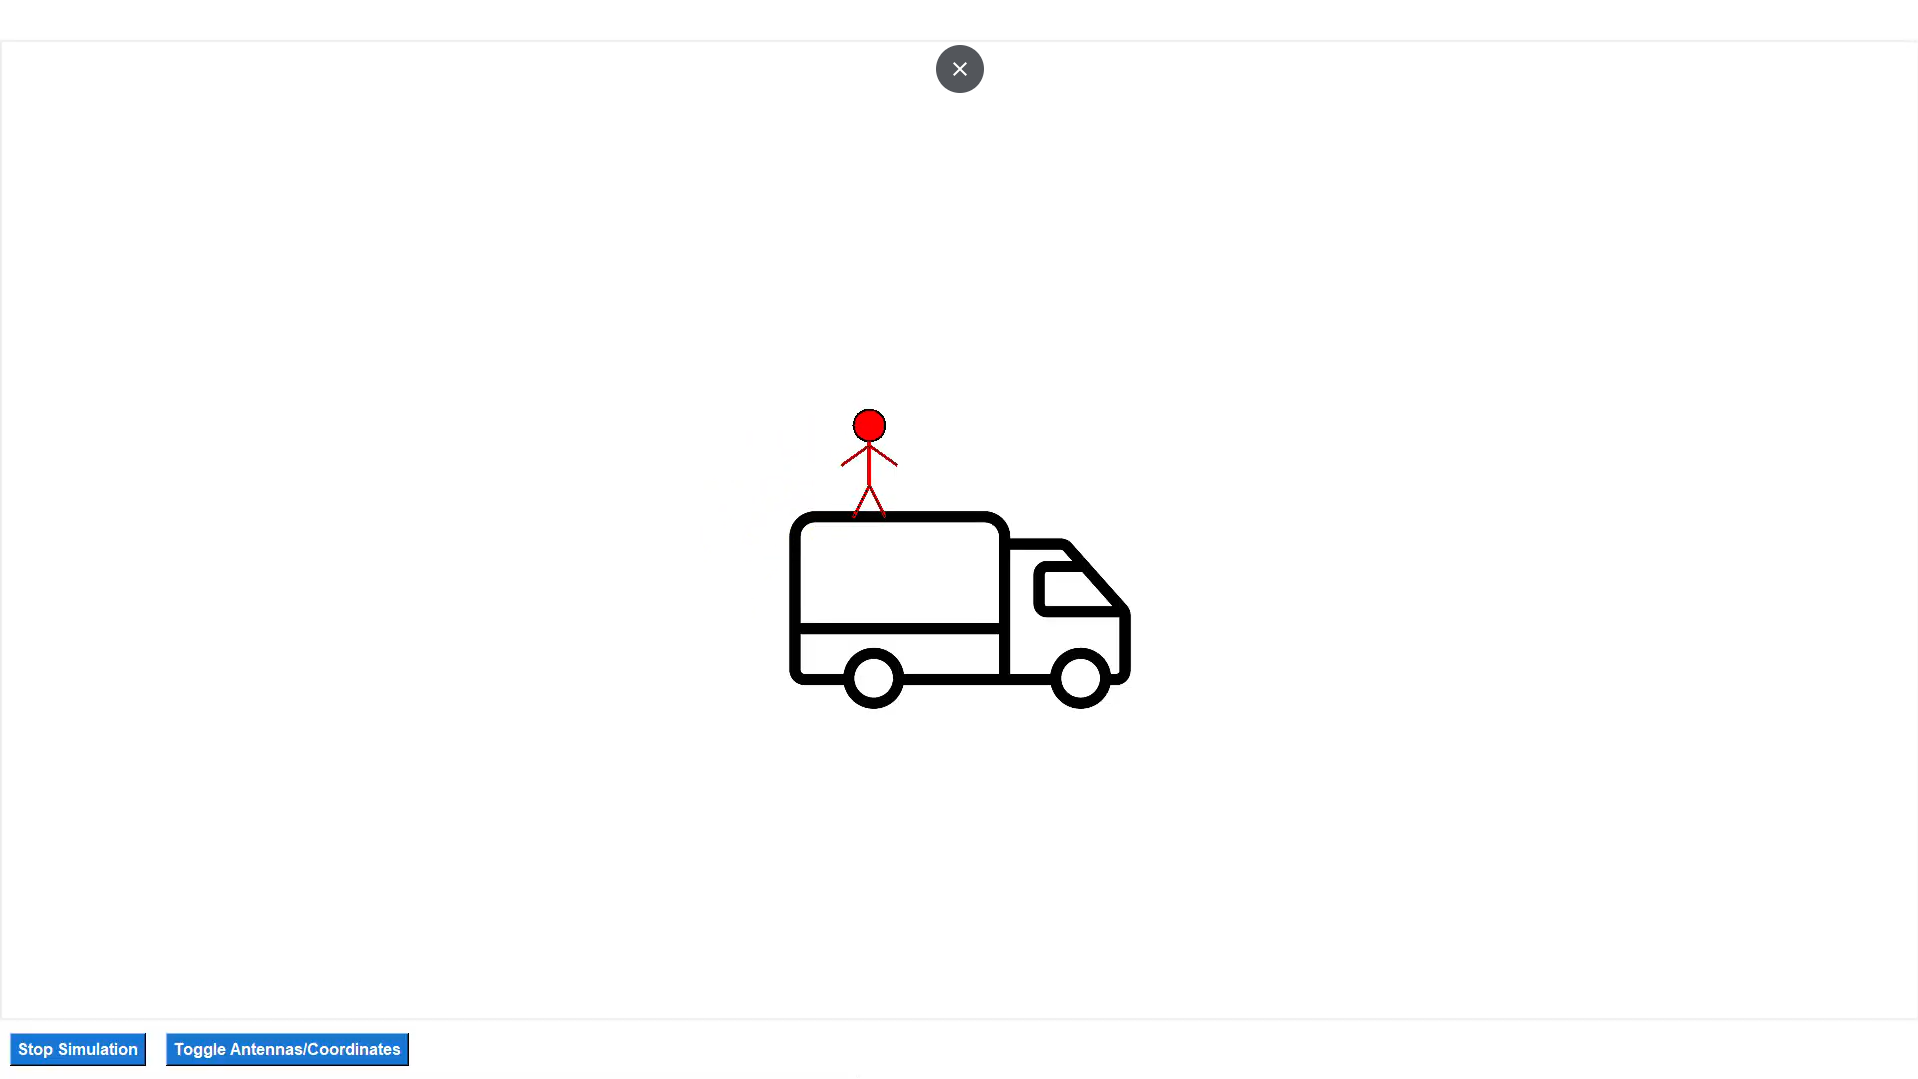
\includegraphics[width=1\linewidth]{images/Minimale Darstellung.png}\\[1ex]
    \centering
    \caption{Minimale Darstellung Benutzeroberfläche \cite{tadic-studienarbeit-ui}}
    \label{ABBILDUNG}
\end{figure}

\paragraph{Zusammenfassung}

Die überarbeitete Visualisierung stellt eine signifikante Verbesserung gegenüber der früheren Version dar. Sie bietet nicht nur eine realitätsnähere 
und dynamischere Darstellung der Position des Tags, sondern erleichtert durch optionale Darstellungselemente und glattere Bewegung auch die Analyse und 
Präsentation für unterschiedliche Zielgruppen. Gleichzeitig wurde Wert auf eine modulare und wartbare Struktur gelegt, sodass zukünftige 
Erweiterungen – etwa die Integration weiterer Visualisierungselemente oder zusätzlicher Sensoren – problemlos möglich sind.

\subsection{Ergebnisse und Benutzerfreundlichkeit}

Die Implementierung der verbesserten Visualisierung zeigt insgesamt funktionale Fortschritte und eine gesteigerte Benutzerfreundlichkeit. Die Anbindung 
über \ac{TCP} funktioniert stabil sowohl im Echtzeitbetrieb mit Live-Messdaten als auch im Offline-Modus über den Datenlogger. Dies ermöglicht eine flexible 
Analyse und Bewertung von Positionsdaten ohne permanenten Zugriff auf die Hardware. Die Integration der Replay-Funktion in die Benutzeroberfläche verläuft
nahtlos – gespeicherte Daten werden zuverlässig geladen, verarbeitet und dargestellt. Dies bietet insbesondere im Entwicklungs- und Testkontext deutliche
Vorteile, da Anpassungen und neue Algorithmen unabhängig von einer aktiven Messumgebung evaluiert werden können.

Im Bereich der Darstellung konnte mit der Ersetzung des bisherigen Tag-Punktes durch eine abstrahierte Stickman-Figur ein deutlicher visueller 
Fortschritt erzielt werden. Zusätzlich wurden Warnstufen eingeführt, welche die Distanz zu einem virtuellen \ac{LKW} durch Farbwechsel (grün, gelb, rot) 
kodieren. Auch die Antennenpositionen und deren Richtungsinformation werden grafisch dargestellt, wenngleich deren Schnittpunkt noch nicht exakt mit der 
berechneten Tag-Position übereinstimmt. Insgesamt ist die Visualisierung deutlich intuitiver und eignet sich besser zur Präsentation auf Fachmessen oder
vor nicht-technischem Publikum. Ein optional zuschaltbares Koordinatensystem erlaubt zudem eine differenzierte technische Auswertung.

Die Bewegung des Tags erscheint derzeit noch leicht ruckartig und verzögert. Es wurden bereits Maßnahmen zur Glättung durch exponentielles Smoothing 
implementiert, allerdings zeigen sich in der Praxis weiterhin Limitierungen, die in zukünftigen Iterationen adressiert werden müssen.

Die Bedienbarkeit der Oberfläche ist insgesamt positiv zu bewerten. Die grafische Benutzeroberfläche zeigt beim Start die relevanten Schaltflächen gut 
sichtbar an. Durch den Toggle-Modus können Darstellungsmodi flexibel gewechselt werden – beispielsweise die Ein- und Ausblendung technischer Hilfslinien. 
Die Benutzerführung ist intuitiv und ermöglicht auch technisch weniger versierten Anwendern eine effiziente Nutzung.

Zusammenfassend lässt sich festhalten, dass die entwickelte Benutzeroberfläche eine stabile Basis für zukünftige Erweiterungen bietet. Neue Features 
können mit überschaubarem Aufwand ergänzt werden, und die vorhandene Architektur erlaubt eine Trennung von Datenaufnahme und Visualisierung. Damit stellt
das System ein praktikables Werkzeug für die Weiterentwicklung, Testung und Demonstration von Assistenzsystemen dar.

\clearpage

\section{Test und Validierung}
\subsection{Testmethodik und -umgebung}

Ziel der Tests war es, die Funktionsweise der entwickelten Komponenten -- insbesondere des Datenloggers und der neuen Visualisierung -- in einer 
realitätsnahen, aber bewusst reduzierten Umgebung zu validieren. Es handelte sich dabei nicht um umfangreiche Praxistests in verschiedensten 
Anwendungsszenarien, sondern um gezielte Funktionstests, die Fehlerquellen aufdecken und Verbesserungspotenziale aufzeigen sollten \cite{myers_testing}.

\paragraph{Testziele}
Im Mittelpunkt stand die Überprüfung folgender Aspekte:
\begin{itemize}
    \item Funktion der Datenerfassung, Speicherung und Wiedergabe im Replay-Modus
    \item Konsistenz der \ac{TCP}-Kommunikation zwischen Logger und \ac{UI}
    \item korrekte Verarbeitung gespeicherter \ac{JSONL}-Daten
    \item visuelle Rückmeldung in der Benutzeroberfläche (z.\,B. Darstellung des Tags, Antennen und Warnfarben)
    \item allgemeine Bedienbarkeit und Reaktion der \ac{UI}-Komponenten \cite{nielsen_usability}
\end{itemize}

\paragraph{Testarten}
Es wurden verschiedene Testarten angewandt:
\begin{itemize}
    \item \textbf{Funktionstests}: Einzelne Module wurden separat geprüft (z.\,B. Speicherung, Wiedergabe, Visualisierung)
    \item \textbf{Integrationstests}: Zusammenspiel von Datenlogger, Netzwerkverbindung und Visualisierung
    \item \textbf{Systemtests}: Gesamtprüfung mit Live- oder gespeicherten Datenströmen
\end{itemize}

\paragraph{Testumgebung}
Die Tests wurden auf einem Standard-PC unter Windows 11 mit Python 3.12 durchgeführt. Die Kommunikation lief lokal über eine \ac{TCP}-Verbindung 
(\texttt{localhost}), was eine stabile Übertragung ohne externe Netzwerkeinflüsse sicherstellte. Als Datenbasis kamen sowohl Live-Messungen mit 
angeschlossener Hardware als auch gespeicherte \ac{JSONL}-Dateien aus früheren Sessions zum Einsatz. Die grafische Benutzeroberfläche wurde dabei im 
Vollbildmodus auf einem 17-Zoll-Bildschirm (Laptop) betrieben.

\paragraph{Ablauf}
Die Tests erfolgten manuell. Zunächst wurde die Verbindung zwischen Logger und UI geprüft. Anschließend wurden verschiedene Datensätze -- sowohl reale
Messungen als auch synthetische Beispiele -- über die \texttt{replayLogger.py \cite{tadic-studienarbeit-ui}} wiedergegeben. Dabei wurde beobachtet, wie die \ac{UI} auf Positionsdaten, 
Sensordaten und Änderungen in der Darstellung reagiert. Auch die neue Funktion zur Darstellung eines Stickmans und des \ac{LKW}-Bildes wurde systematisch 
getestet. Der Wechsel des Darstellungsmodus (z.\,B. Ein-/Ausblenden der Achsen) wurde ebenfalls geprüft.

Ergänzend dazu wurde gezielt versucht, typische Grenzsituationen und Extremszenarien zu simulieren. Dazu gehörten beispielsweise sehr schnelle oder 
sehr langsame Bewegungen des Tags sowie Positionen am äußersten linken oder rechten Rand des Koordinatensystems. Ziel war es zu prüfen, ob die 
Positionsberechnung, Visualisierung und Stabilität auch in diesen Randbereichen erwartungsgemäß funktionieren.

\paragraph{Einschränkungen}
Aufgrund zeitlicher und infrastruktureller Begrenzungen wurde auf umfangreiche Feldversuche oder Szenarien im Realbetrieb verzichtet. Ziel 
war primär eine funktionale Prüfung der neu entwickelten Komponenten. Eine tiefgreifende Evaluierung im produktiven Umfeld ist für spätere 
Projektphasen vorgesehen.

\subsection{Ergebnisse der Tests}

Die durchgeführten Tests hatten zum Ziel, die grundsätzliche Funktionalität des entwickelten Datenloggers sowie der erweiterten Visualisierung zu 
überprüfen. Dabei standen insbesondere Aspekte wie Datenintegrität, Kommunikation, Benutzerfreundlichkeit und visuelle Darstellung im Vordergrund.

\paragraph{Funktionalität und Kommunikation}
Die Tests zeigten, dass die Speicherung der erfassten Sensordaten im \ac{JSONL}-Format zuverlässig funktioniert. Auch die Wiedergabe der gespeicherten Daten 
im Replay-Modus über \texttt{replayLogger.py \cite{tadic-studienarbeit-ui}} erwies sich als stabil. Die \ac{TCP}-Kommunikation zwischen Datenlogger und grafischer Benutzeroberfläche konnte 
ohne Verbindungsabbrüche oder Datenverluste durchgeführt werden. Es war möglich, sowohl reale Messdaten als auch gespeicherte Daten aus dem Logger 
erfolgreich in die Benutzeroberfläche zu laden.

\paragraph{Darstellung des Tags}
Die Bewegung des Tags innerhalb der grafischen Oberfläche erwies sich noch als verbesserungsbedürftig. Obwohl bereits ein Glättungsalgorithmus 
implementiert wurde, wirkt die Bewegung weiterhin leicht verzögert und ruckartig. Besonders bei Extrempositionen – also wenn sich der Tag weit 
rechts oder links außerhalb des zentralen Bereichs bewegt – konnte beobachtet werden, dass die Ortung deutlich an Genauigkeit verliert. Dies liegt
am zugrunde liegenden Triangulationsverfahren: Wenn sich beide gemessenen Winkel stark überlagern, ist eine exakte Positionsbestimmung kaum noch 
möglich \cite{thurmond2001point}.

\begin{figure}[H]
    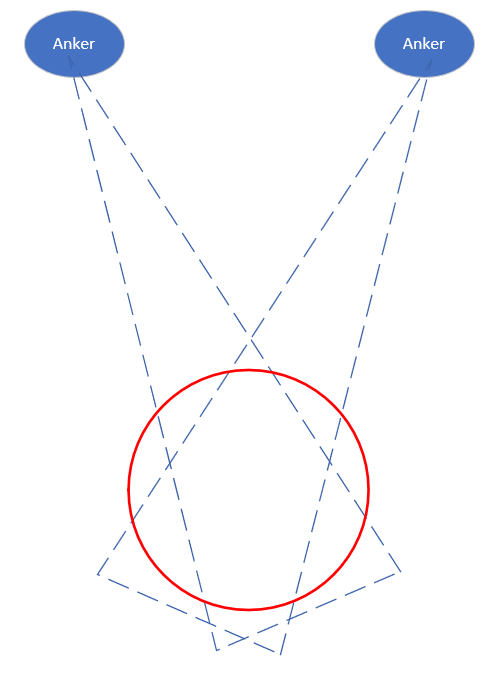
\includegraphics[width=0.5\linewidth]{images/Gute Triangulation.png}\\[1ex]
    \centering
    \caption{Gute Triangulation \\
                Quelle:Eigene Darstellung}
    \label{ABBILDUNG}
\end{figure}

\clearpage

\begin{figure}[H]
    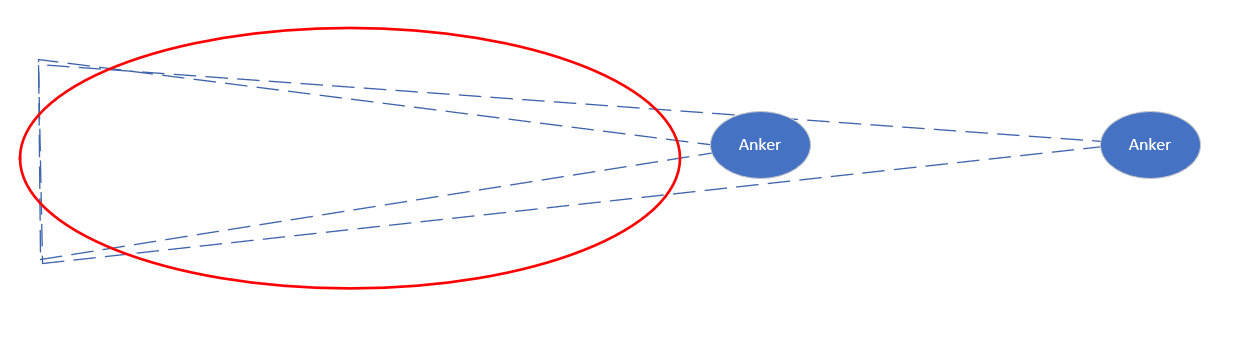
\includegraphics[width=1\linewidth]{images/Schlechte Triangulation.png}\\[1ex]
    \centering
    \caption{Schlechte Triangulation \\
            Quelle:Eigene Darstellung}
    \label{ABBILDUNG}
\end{figure}

\paragraph{Visualisierung und Layout}
Die Darstellung wurde im Vergleich zum vorherigen Zustand deutlich verbessert. Anstelle eines einfachen Punktes wird der Tag nun als stilisierter 
Stickman visualisiert. Darüber hinaus wurde ein \ac{LKW}-Bild zur Verdeutlichung der Anwendungssituation ergänzt. Die Antennenpositionen werden 
grafisch dargestellt und mit Richtungslinien versehen, welche sich in den meisten Fällen korrekt im Bereich der ermittelten Position schneiden – ein 
klares visuelles Feedback über die Funktionsweise des Systems. Dennoch bleibt die Darstellung grundsätzlich einfach gehalten. Zusätzliche 
Visualisierungselemente wie eine Geschwindigkeitsanzeige, eine dynamische Skalierung des Bewegungsraums oder realistischere Proportionen der 
dargestellten Objekte könnten künftig integriert werden.

\paragraph{Benutzerfreundlichkeit}
Die Benutzeroberfläche erwies sich in der Praxis als einfach zu bedienen. Beim Starten des Programms werden klar beschriftete Schaltflächen angezeigt, 
die ohne Vorkenntnisse verständlich sind. Funktionen wie das Starten und Stoppen der Simulation oder das Umschalten von Koordinaten- und Antennenanzeige 
sind intuitiv zugänglich. Die Implementierung der \acf{BAT}-Datei zum Start des Datenloggers erleichtert zusätzlich die Bedienung, insbesondere für unerfahrene
Nutzer \cite{nielsen_usability}. Zudem kann zwischen verschiedenen gespeicherten Messreihen gewählt, diese umbenannt und erneut abgespielt werden.

\paragraph{Zusammenfassende Bewertung}
Insgesamt wurde mit dem entwickelten System ein funktionaler Prototyp geschaffen, der die gewünschten Kernfunktionen erfüllt. Die Integration des 
Datenloggers in die bestehende Softwareumgebung ist gelungen und erlaubt eine flexible Nutzung, sowohl online als auch offline. Die Visualisierung 
ist verständlicher als zuvor, besonders im Hinblick auf Präsentationen und Messen. Dennoch bestehen in mehreren Bereichen Potenziale zur weiteren 
Optimierung, insbesondere in der flüssigen Bewegung des Tags, in der Genauigkeit der Darstellung sowie in der Erweiterung des visuellen Feedbacks für
komplexere Anwendungsszenarien.

\subsection{Diskussion der Testergebnisse und Optimierungspotentiale}

Die durchgeführten Funktionstests zeigen, dass die wesentlichen Kernziele – insbesondere die prototypische Realisierung des Datenloggers und 
dessen Anbindung an die Visualisierung – erfüllt wurden. Dennoch offenbaren die Testergebnisse mehrere Schwachstellen und Hinweise auf künftigen 
Verbesserungsbedarf, die im Folgenden diskutiert werden.

\paragraph{Limitierungen in der Positionsdarstellung}

Trotz implementierter Glättungsmechanismen bleibt die Bewegung des Tags auf der Benutzeroberfläche merklich ruckartig. Insbesondere bei 
schnellen Richtungswechseln oder Bewegungen am Rand des Koordinatensystems treten Verzögerungen auf. Dies kann auf die gewählten Smoothing-Parameter 
oder das einfache Exponentialfilter-Verfahren zurückgeführt werden, das bei dynamischen Bewegungen an seine Grenzen stößt. Eine adaptive Glättung, die 
sich an der Bewegungsgeschwindigkeit orientiert, könnte hier künftig Abhilfe schaffen.

Ein weiterer kritischer Punkt ist die eingeschränkte Genauigkeit der Positionsbestimmung bei extremen Positionen. Wenn sich der Tag sehr weit 
links oder rechts außerhalb der Hauptmessachse befindet, versagt die Triangulation teilweise. Der Grund liegt in der Geometrie der \ac{AoA}-Messung: 
Bei annähernd parallelen Winkelmessungen zweier Anker wird der Schnittpunkt der Geraden numerisch instabil, was eine präzise Lokalisierung erschwert \cite{thurmond2001point}.

\paragraph{Darstellung und Interpretation der Ergebnisse}

Die Visualisierung wurde gegenüber der ursprünglichen Version deutlich verbessert. Die Einführung eines symbolischen Stickman-Modells sowie 
eines schematischen \ac{LKW}-Bildes erhöht die Verständlichkeit, besonders für externe Zielgruppen oder Präsentationen. Gleichzeitig bleibt die 
grafische Ausgestaltung noch rudimentär. Elemente wie Maßstabsanzeige, Bewegungsverläufe, Risikozonen oder Geschwindigkeitspfeile fehlen bislang, 
könnten aber die Interpretation der Szenarien erheblich erleichtern.

Darüber hinaus könnte auch die Proportionalität zwischen realer Bewegung und Koordinatensystem verbessert werden. Aktuell ist die Zuordnung zwischen 
physischer Verschiebung und grafischer Darstellung nicht intuitiv nachvollziehbar, was insbesondere bei der Validierung der Messergebnisse hinderlich 
sein kann.

\paragraph{Bedienbarkeit und Nutzbarkeit}

Die Bedienung der Visualisierungsoberfläche gestaltet sich insgesamt benutzerfreundlich. Die eingefügten Steuerungselemente (z.\,B. Toggle-Schalter 
für die Darstellung der Koordinatenachsen) sowie die Möglichkeit, das Programm per \texttt{.bat}-Datei zu starten, erleichtern die Nutzung auch für 
weniger erfahrene Anwender. Die einfache Darstellung ist für erste Tests und Demonstrationen durchaus ausreichend, lässt sich jedoch hinsichtlich 
Detailtiefe und Flexibilität weiterentwickeln.

\paragraph{Potenziale zur Erweiterung}

Für die Weiterentwicklung ergeben sich mehrere sinnvolle Ansätze. Neben einer grafischen Verfeinerung könnten folgende Maßnahmen zur 
Optimierung beitragen:

\begin{itemize}
    \item Einführung eines dynamischen Zoom- oder Perspektivmodus zur besseren Verfolgung der Tag-Bewegung
    \item Erweiterung der Darstellung um Geschwindigkeit, Bewegungsrichtung und Unsicherheitsbereiche
    \item Modularisierung der Visualisierung zur einfacheren Einbindung weiterer Objekte oder Assistenzsysteme
    \item Verbesserung der Glättungslogik mit adaptiven oder maschinellen Verfahren
    \item Vorbereitung auf künftige Erweiterungen wie eine 3D-Ansicht
\end{itemize}

\paragraph{Fazit}

Die bisherigen Testergebnisse zeigen eine solide Basis, auf der sich weiter aufbauen lässt. Sowohl die technische Funktionalität als auch die visuelle
Vermittlung der Daten sind grundsätzlich gegeben, müssen jedoch für eine belastbare Systembewertung und breitere Nutzbarkeit noch weiterentwickelt und 
verfeinert werden.

\clearpage

\section{Kritische Bewertung und Ausblick}
\subsection{Reflexion der erreichten Ergebnisse}

Im Rahmen dieser Arbeit wurde das Ziel verfolgt, ein robustes Datenloggersystem zu entwickeln sowie die bestehende Visualisierung einer 
Bluetooth-\ac{AoA}-basierten Lokalisierungslösung gezielt zu erweitern. Rückblickend lässt sich feststellen, dass wesentliche Kernziele erfolgreich 
umgesetzt wurden.

Der entwickelte Datenlogger ermöglicht eine strukturierte und flexible Erfassung sowie Speicherung von Messdaten im \ac{JSONL}-Format. Er erlaubt eine 
spätere Wiedergabe der Daten ohne Hardwareeinsatz und schafft somit eine effektive Grundlage für Tests, Parametrierung und Algorithmenentwicklung. 
Die Integration des Loggers in die bestehende Softwareumgebung erfolgte reibungslos durch ein separates Python-Skript mit minimalen Änderungen am 
Ursprungscode. Auch die Konnektivität zur Benutzeroberfläche über eine \ac{TCP}-Verbindung funktionierte stabil, sowohl im Live-Betrieb als auch im 
Replay-Modus.

Auf Seiten der Visualisierung wurde die bisher sehr reduzierte Darstellung um mehrere Elemente erweitert. Die Verwendung eines stilisierten 
Stickman-Modells zur Repräsentation des Tags, die Einbindung eines realitätsnahen \ac{LKW}-Bildes sowie die farbliche Warnstufendarstellung 
führten zu einer deutlich verständlicheren und praxistauglicheren Repräsentation. Dies ist insbesondere im Hinblick auf externe Präsentationen, 
z.\,B. auf Messen oder Präsentationen, ein entscheidender Vorteil.

Trotz dieser Fortschritte zeigen sich auch einige Grenzen. Die Bewegung des Tags ist nach wie vor leicht verzögert und nicht vollständig flüssig, 
obwohl bereits erste Maßnahmen zur Glättung implementiert wurden. In Randbereichen des Messfeldes stößt die Triangulation durch sich überlappende 
Winkelpaare an ihre mathematischen Grenzen, was zu ungenauen oder nicht vorhandenen Positionsschätzungen führt. Auch die visuelle Darstellung – etwa in 
Bezug auf Maßstäblichkeit oder ergänzende Informationen wie Geschwindigkeit – bietet weiteres Verbesserungspotenzial.

Nichtsdestotrotz konnte durch die modulare Struktur, den Einsatz etablierter Technologien (Python, \ac{JSON}, \ac{TCP}) sowie den pragmatischen Ansatz ein 
funktionierendes System geschaffen werden, das die Grundlage für weiterführende Entwicklungen bietet. Die Arbeit zeigt damit deutlich, dass durch 
gezielte Ergänzungen und strukturiertes Vorgehen auch in einer begrenzten Projektlaufzeit signifikante Fortschritte in Funktionalität und 
Benutzerfreundlichkeit erzielt werden können.

\subsection{Grenzen der aktuellen Umsetzung}

Trotz der erfolgreichen Umsetzung eines funktionalen Datenloggers und einer verbesserten Visualisierung bestehen derzeit noch mehrere Einschränkungen, 
die das System in seiner Einsatzbreite und Qualität begrenzen.

\paragraph{Begrenzte Genauigkeit der Positionsbestimmung} 
Die Positionsschätzung des Tags basiert auf Triangulation aus den gemessenen \ac{AoA}-Winkeln zweier Anker. Dieses Verfahren liefert nur dann 
zuverlässige Ergebnisse, wenn die geometrische Anordnung der Anker günstig gewählt ist. Besonders bei Messungen an den Rändern des definierten 
Messfelds (z.\,B. weit links oder rechts) kann es aufgrund der Überlagerung oder Parallelität der Winkellinien zu ungenauen oder gar nicht 
berechenbaren Positionen kommen.

\paragraph{Nicht vollständig realitätsgetreue Bewegungsdarstellung}
Obwohl Maßnahmen zur Glättung der Bewegung (z.\,B. mittels Pufferung und Smoothing) umgesetzt wurden, wirkt die Visualisierung des bewegten 
Tags weiterhin leicht ruckartig und reagiert nicht in Echtzeit. Zudem fehlt derzeit eine maßstabsgetreue Übertragung der tatsächlichen Bewegung 
auf die Bildschirmanzeige.

\paragraph{Einfaches visuelles Layout}
Die Visualisierung nutzt bisher einfache grafische Elemente wie einen stilisierten Stickman und ein eingefügtes Bild eines \ac{LKW}s. 
Die Darstellung unterstützt die Verständlichkeit, lässt jedoch hinsichtlich Detailtiefe, Ästhetik und Interaktivität noch deutlichen Spielraum 
für Verbesserungen. Eine Möglichkeit zur perspektivischen Darstellung, Animation komplexerer Objekte oder eine interaktive Benutzersteuerung ist 
bislang nicht vorgesehen.

\paragraph{Begrenzte Testtiefe}
Die entwickelte Lösung wurde im Rahmen kleinerer Testszenarien mit kurzer Laufzeit erprobt. Umfangreiche Testreihen unter realitätsnahen 
Bedingungen – etwa mit komplexer Bewegung, Störeinflüssen oder Mehrpersonen-Szenarien – konnten zeitbedingt nicht durchgeführt werden.

\paragraph{Fehlende erweiterte Analyse- und Mehrbenutzerfunktionen}
Die aktuelle Implementierung erlaubt eine visuelle Einzelnutzung mit Echtzeitdarstellung bzw. Offline-Replay. Weiterführende Funktionalitäten wie 
gleichzeitiger Mehrbenutzerzugriff, interaktive Analysewerkzeuge, Exportfunktionen oder statistische Auswertungen (z.\,B. Heatmaps) sind derzeit nicht 
enthalten.

\paragraph{Technische Einschränkungen der Visualisierung}
Die Umsetzung der Benutzeroberfläche auf Basis von Python und Tkinter bringt den Vorteil einer schnellen Realisierbarkeit, schränkt jedoch die 
grafischen und performanten Möglichkeiten ein. Zudem erfordert der Datenlogger eine strukturierte Ablage der \ac{JSONL}-Dateien und Pfade, was die 
Portabilität des Systems derzeit noch begrenzt.

Diese Punkte zeigen klar auf, in welchen Bereichen gezielte Weiterentwicklungen erforderlich sind, um das System robuster, skalierbarer und 
praxistauglicher zu gestalten.

\subsection{Vorschläge für zukünftige Weiterentwicklungen}

Basierend auf den Ergebnissen und Erkenntnissen der bisherigen Arbeit ergeben sich verschiedene Ansatzpunkte für eine sinnvolle Weiterentwicklung
des entwickelten Systems.

\paragraph{Technische Optimierung der Bewegungsglättung}
Die Bewegung des Tags ist in der aktuellen Visualisierung noch nicht ausreichend flüssig. Obwohl bereits ein Kalman-basiertes Glättungsverfahren 
implementiert wurde, treten weiterhin ruckartige Darstellungen und spürbare Verzögerungen auf. Eine Verbesserung kann erzielt werden, indem die 
Kalman-Parameter – etwa Prozess- und Messrauschen – adaptiv angepasst und feiner auf die Dynamik des Systems abgestimmt werden, um eine realitätsnähere
 Bewegung des Tags zu erreichen \cite{kalman_filter_book}.

\paragraph{Verbesserung der Triangulation bei Randlagen}
Ein beobachtetes Problem betrifft die Genauigkeit der Positionsbestimmung, insbesondere wenn sich das Tag am Rand des Erfassungsbereichs befindet. 
Hierbei treten geometrische Probleme auf, da die beiden Winkelmessstrahlen nahezu parallel verlaufen und die Schnittpunktbestimmung ungenau wird. 
Eine Möglichkeit zur Verbesserung besteht in der Integration eines dritten Antennen-Boards. Durch die zusätzliche Winkelmessung kann die geometrische 
Ambiguität reduziert und die Lokalisierungsgenauigkeit signifikant gesteigert werden.

\paragraph{Erweiterung der Replay-Funktionalität}
Der Datenlogger erlaubt bereits das Abspielen aufgezeichneter Messdaten. In zukünftigen Versionen könnte diese Funktion erweitert werden, um Parameter 
direkt über eine grafische Benutzeroberfläche anpassen zu können. Eine visuelle Konfigurationsmaske mit Live-Feedback würde die Entwicklungs- und 
Testphase erheblich vereinfachen.

\paragraph{Erweiterung der Visualisierungsmöglichkeiten}
Die Visualisierung des Tags wurde bereits durch einen stilisierten Stickman sowie ein \ac{LKW}-Modell ergänzt. Um jedoch noch realitätsnähere und
professionellere Darstellungen zu ermöglichen – insbesondere bei öffentlichen Vorführungen oder Messen – könnten 3D-Modelle eingesetzt werden. 
Auch zusätzliche visuelle Indikatoren wie Bewegungstrails, Heatmaps oder Geschwindigkeitssymbole wären denkbar \cite{webgl_book}.

Zudem könnte das Koordinatensystem um interaktive Funktionen wie Zoom, Skalierung oder Ein-/Ausblendung erweitert werden. Mittelfristig wäre auch 
der Umstieg auf eine leistungsfähigere Visualisierungsplattform, etwa auf Basis von Unity3D oder WebGL, zu evaluieren \cite{buyuksalih20173d}.

\paragraph{Verbesserung der Benutzeroberfläche}
Die aktuelle \ac{UI} bietet bereits eine grundlegend benutzerfreundliche Bedienung. Zukünftig wäre jedoch eine webbasierte Variante wünschenswert, 
die plattformunabhängig funktioniert und auch über mobile Endgeräte steuerbar ist. Eine intuitive Konfiguration von Replay-, Logging- und 
Visualisierungsparametern würde die Nutzerfreundlichkeit zusätzlich steigern \cite{ux_design_book}.

\paragraph{Tests und Validierung}
Die durchgeführten Tests waren in ihrem Umfang noch begrenzt. Für zukünftige Weiterentwicklungen sollte ein strukturierter Testkatalog 
entwickelt werden, der typische Anwendungsszenarien, Grenzfälle und Langzeittests umfasst. Dadurch ließe sich die Robustheit und Zuverlässigkeit 
der Lösung weiter erhöhen.

\paragraph{Systemintegration und Modularisierung}
Langfristig wäre eine stärkere Modularisierung der Softwarestruktur anzustreben. Durch eine saubere Trennung von Datenaufnahme, Auswertung, 
Visualisierung und Replay-Modulen ließe sich die Wartbarkeit verbessern. Auch die Integration externer Sensoren oder Cloud-Plattformen zur 
weitergehenden Analyse könnte über standardisierte Schnittstellen ermöglicht werden \cite{software_architecture_modular}.

\paragraph{Zusammenfassung}
Insgesamt existieren vielfältige Ansatzpunkte für die Weiterentwicklung der Lösung. Diese reichen von technischen Verbesserungen der 
Positionsbestimmung und Visualisierung über benutzerfreundliche \ac{UI}-Konzepte bis hin zur Erweiterung des Hardware-Setups durch zusätzliche Anker. 
Gerade die Kombination dieser Maßnahmen verspricht eine deutliche Steigerung der Systemqualität und Anwendbarkeit in praxisnahen Einsatzszenarien.

\clearpage

%---------------------------------------------------------
% Bibliografie
%---------------------------------------------------------
\begingroup
\sloppy
\nocite{*}
\printbibliography

\end{document}
